Previously, I showed that different phonological and morphological phenomena can be modeled as subregular languages.
In this chapter, I demonstrate the automatic extraction of subregular languages from linguistic data.
To do so, I employ four subregular language classes that express generalizations, including local and long-distance dependencies such as attested and unattested harmony systems with and without blockers, word-final devoicing, and even suprasegmental patterns.

Indeed, local patterns can be expressed with strictly local (SL) grammars and long-distance phenomena with strictly piecewise (SP) grammars.
If a long-distance pattern uses blockers (e.g., opaque vowels in vowel harmony), then we use tier-based strictly local (TSL) grammars.
If the language exhibits multiple long-distance phenomena, then we may also need  multi-tier strictly local (MTSL) grammars.
This perspective on morphotactics and phonotactics also rules out typologically unattested patterns such as first-last harmony, majority harmony, or embedded circumfixation.

In what follows, I discuss algorithms which extract SL, SP, TSL and MTSL grammars from the data.
Apart from the training sample, these algorithms require knowing the class of the target grammar, and the locality window of that grammar, i.e.\ the length of substructures with which it operates.
In other words, we need to know the formal complexity of the target language in order to learn it efficiently using subregular learning algorithms.
Given a sufficient and representative training sample and proper specifications of the target grammar, the subregular learners discover the pattern in polynomial time and data.

I start by introducing the datasets that I will use throughout the chapter to perform the learning experiments.
These datasets vary from automatically generated artificial languages to real wordlists exemplifying attested linguistic dependencies, such as word-final devoicing in German, vowel harmony in Turkish, and others.
I then use these datasets as training samples for the subregular learners, discuss the obtained grammars, and automatically evaluate the predictions of those grammars based on the well-formedness of the strings they generate.
At the end of the chapter, I provide a table that summarizes the results of the learning experiments.

The exemplified learners work exclusively with \emph{string representations}.
These algorithms focus on structural properties; they are limited to non-probabilistic algorithms which evaluate the well-formedness of input strings.
As of now, I have not implemented statistical versions of these algorithms, or algorithms which work with non-string-based representations.


The subregular learners, scanners and sample generators are available as a module of my Python package \emph{SigmaPie} \href{https://pypi.org/project/SigmaPie/}{\faCube} \citep{sigmapie}.
The code of the toolkit is provided in Appendix A.
It is also available on GitHub, as well as the code behind the implementations of the further discussed learning experiments \href{https://github.com/alenaks/subregular-experiments}{\faGithub} \citep{GHsubex}.


\section{The experimental setup}

I use both artificial and natural languages to explore the performance of the SL, SP, TSL and MTSL learners.
The artificial languages imitate concrete natural language phenomena.
The learning of these artificial languages shows us if the extraction of those patterns is possible \emph{conceptually}, whereas the performance of those algorithms on the natural language datasets shows us what is currently possible \emph{in practice}.
Due to the transparency and interpretability of the subregular learners, we can always see the path the learner took to extract the target grammar.
If the learning experiment was unsuccessful, we can always look inside those algorithms and see what obstructed the convergence.

\subsection{Experimental pipeline}

The \textbf{experimental pipeline} involved $3$ steps: learning, generation, and evaluation.
\textbf{Learning} included automatic extraction of subregular grammars from the given training samples.
I then used those extracted grammars to \textbf{generate} samples of strings.
Finally, during the \textbf{evaluation} step, I computed the percentage of the strings from the automatically generated datasets that are well-formed with respect to the target grammars.

Regardless of what can be considered a general practice, I am \emph{not} testing the performance of the grammars on the held out parts of the training sample.
That approach would not let us to detect the cases in which the learner ``overgeneralized'' the pattern.
For example, some learning experiments resulted in the learner incorrectly converging on the empty negative grammar: such a learner simply assumed that ``anything goes''.
Trivially, it will score $100$\% on all the held-out data.
Only by looking at the predictions of the grammar it is possible to see if the learner generalized the language of the training sample.

The results showing the performance of the subregular models are presented in \ref{interimsummarylanguages}.
Only negative grammars were employed for the experiments due to the succinctness of their grammars.


\subsection{Natural languages}

The real data used for the experiments comes from German, Finnish and Turkish.
The German dataset is a wordlist for wordgames posted by \texttt{enz} \href{https://github.com/enz/german-wordlist}{\faGithub} \citep{GHenz}.
The Finnish data is taken from a collection of wordlists scraped by \texttt{douglasbuzatto} \href{https://github.com/douglasbuzatto/WordLists}{\faGithub} \citep{GHdouglasbuzatto}.
The collection of Turkish words was uploaded by \cite{HarrisonEtAl2004} as a part of his project \emph{The Vowel Harmony Calculator} \href{http://www.swarthmore.edu/SocSci/harmony/public_html/dummyresults.html}{\faChain}.
Due to the non-probabilistic nature of the algorithms, I removed the data items that violate the target generalizations, such as disharmonic stems.
This is necessary to evaluate the structural properties of the learners.
In the future, the availability of the probabilistic subregular learners will allow to process disharmonic stems as well.

The target patterns exemplified by natural language datasets involved three levels of abstraction.
The \emph{raw representations} contained the strings from the wordlists; it allows us to explore the problems that the learner faces when it is given realistic data.
The \emph{masked representation} is more abstract and involved substituting all the symbols in the original data that are not relevant for the target pattern by a single symbol of choice.
It allows the learner to focus on the generalization since all the ``irrelevant'' material is masked.
It lets us explore if there is enough information in the simplified strings of the language to notice the pattern behind the behavior of the dependent elements.
For example, if Turkish vowel harmony was explored under this perspective, all consonants were masked as $x$.
Finally, the \emph{abstract representation} represented the pattern with the highest degree of generality, therefore compelling the learner to discover only the ``core'' part of the generalization.
This allows us to carefully examine the learning process: the levels of abstraction help remove the ``concreteness'' of the natural language dependencies and focus on the general properties of the target patterns.


\subsection{Artificial languages}
\label{secartlang}

I used $5$ artificial language generators for the experiments in this and the following chapters. Their code is available on GitHub \href{https://github.com/alenaks/subregular-experiments}{\faGithub} \citep{GHsubex}.
In all of these generators, the number of strings (the default value is $10$) and the length of those strings (the default value is also $10$) can be defined a priori.


The \textbf{Simple Harmony Generator} encodes and generates samples demonstrating long-distance dependencies such as vowel harmony and consonant harmony.
The generator lets us define several harmonic classes, where a \emph{harmonic class} is a collection of elements that cannot co-occur within the same well-formed word of the language.
For example, if there are two harmonic classes $A = \{a, o\}$ and $B = \{b, p\}$, the well-formed words of this language can use at most $1$ element of these class, unless a blocker intervenes.
These classes $A$ and $B$ define strings such as \emph{apappa}, \emph{oppooo}, \emph{bbaab}, and so on; but the ones such as \emph{abbobb} cannot be produced by this generator.
The blockers are defined as $\{f$:$a, s$:$p\}$, meaning that the occurrence of $f$ in the string allows only $a$ to be seen after itself.
Other elements of $a$'s harmonic class are now prohibited, e.g., $f$ blocks any subsequent $o$.
Additionally, $b$ is prohibited after an $s$.
This generator now produces words such as \emph{ababb\textbf{s}appp} and \emph{obbo\textbf{f}ba\textbf{s}aapp}.
Transparent elements can be expressed as single-item harmonic classes, such as $X = \{x\}$; it lets $x$ be freely inserted in different parts of any string.
Additionally, the minimal and maximal length of every harmonic class is also parametrized (the default values are $\textrm{min} = 1$ and $\textrm{max} = 3$), as well as the emission probability of every blocker (the default probability is $p(s) = p(f) = 0.2$).


The \textbf{Fake Turkish Generator} is much more specialized in comparison to the generator outlined above.
It produces sequences of vowels that are well-formed with respect to the rules of Turkish vowel harmony, with all the consonants simplified to a single symbol.
Like that, it produces harmonic sequences such as \emph{\"ox\"u\"uxeei} and \emph{oa\textsci xxx\textsci\textsci}.
The ``choice'' of the consonant, as well as the minimal and maximal lengths of vowel and consonant clusters, can be specified in the generator.
The Turkish dataset cannot be defined by the Simple Harmony Generator because the same set of segments participates in two types of harmonies (backness and rounding), and some of the vowels that are undergoers for the backness harmony serve as blockers for the rounding one.


The \textbf{Word-Final Devoicing Generator} simply produces a set of strings that follow the rule of the word-final devoicing.
For this, we define a list of voiced and voiceless segments, as well as the alphabet of the language.
By default, the voiced and voiceless segments are $\{b\}$ and $\{p\}$ respectively, and the alphabet of the language is $\{a, b, p\}$.
For example, this generator produces strings such as \emph{apabaa} and \emph{abbap}, but never the ones such as \emph{paab}.


The \textbf{UTP Generator} produces strings of low ($L$) and high ($H$) tones that are well-formed concerning the unbounded tonal plateauing (UTP) generalization in Luganda.
This generalization prohibits a low tone from appearing in a string if surrounded by high tones.
For example, it produces strings such as \emph{LLHH} and \emph{LHHHL}, but is incapable of generating the ones such as \emph{HHLHH} and \emph{HLLLH}.


The \textbf{First-Last Harmony Generator} generates a language with first-last harmony.
The language enforces agreement between the first and the last elements within the string.
A list of agreeing elements needs to be specified (the default value is $\{a, o\}$), as well as the list of all other elements that can appear in the well-formed strings of this language ($\{a, o, x\}$ is the default).
Strings such as \emph{axoxoxa} and \emph{ooaxo} are then grammatical, but \emph{axaxxo} or \emph{oaa} are not.
Importantly, harmonic systems of this type are unattested in natural languages.%
\footnote{First-last harmony can be unattested due to several different reasons.
It might be impossible for such a pattern to naturally occur from language changes, or it can simply be not learnable by humans.
\cite{Lai15} discusses the differences between the attested and unattested harmony patterns.}

These generators were employed to produce data that was then fed to the SL, SP, TSL and MTSL learners.
The next subsection provides the detailed description of the datasets used as training samples during the subregular experiments.


\subsection{Target patterns}

The learning experiments in this chapter target typologically widespread linguistic patterns such as word-final devoicing, tone plateauing and harmonic systems of different kinds.
Here, I explain how I obtained the artificial training samples for every one of these patterns.
For German, Finnish and Turkish natural language datasets, I also discuss the preprocessing steps that I did to get the data in the shape appropriate for the experiments.


\subsubsection{Pattern 1: word-final devoicing}

The phenomenon of word-final devoicing is attested in languages such as Russian and German.
It prohibits underlyingly voiced obstruents from being pronounced voiced at the end of the word.
In German, word-final /b/, /d/, and /g/ are realized as [p], [t], and [k] \citep{Wiebke1995}.
For example, the word for `children' is \emph{Kinder}, but its singular form is pronounced as \emph{Kin[t]}, i.e.\ the underlyingly voiced segment is realized as voiceless at the end of the word.

For this experiment, I used a German wordlist \href{https://github.com/enz/german-wordlist}{\faGithub} \citep{GHenz}, its masked version, and an abstract representation of this pattern.
During the masking step, all irrelevant segments were simply represented as $a$, and the abstract representation of this pattern only included $3$ types of elements: voiced obstruents ($b$), voiceless obstruents ($p$), and others ($a$).

\paragraph{Raw representation}

This wordlist in its original form contains $685,618$ words written in German orthography.
However, German orthography does not reflect the process of the word-final devoicing and therefore the preprocessing of this corpus was necessary.
It included two steps: incorporating the effect of the word-final devoicing and filtering words that contain non-German symbols.
Firstly, I substituted every occurrence of the word-final /g/, /b/ and /d/ by their voiceless counterparts /k/, /p/, and /d/, respectively.
In total, there were $1,599$ words that end with /b/ ($0.2$\% of the total number of words); $15,294$ words that end with /d/ ($2.2$\%); and $17,098$ words with a word-final /g/ ($2.4$\%).
This step resulted in words such as \emph{Kind} being changed to \emph{Kint}, \emph{Rad} to \emph{Rat}, etc.
Secondly, I excluded all strings that use letters that do not belong to the German alphabet, such as \emph{z\textbarl oty}, \emph{ch\^ateau}, and some others.
After those words were excluded, the size of the German wordlist became $685,147$ words.
%The post-processed German sample is further referred to throughout this chapter as \texttt{german\_wfd}.

\begin{lstlisting}[language=Python]
print(german_wfd)
# ['hochjagende', 'zugebliebener', 'verbricht', 'besuchszimmer', 'beschneien', ...]
\end{lstlisting}


\paragraph{Masked representation}

The next step was to simplify German wordlist.
Namely, for the phenomenon of the word-final devoicing, segments other than $\{b, p, g, k, d, t\}$ are not important, and therefore all of them can be simply masked as $a$.
The rules of the masking are summarized in Table \ref{germanmap1}.
Since none of the words were deleted during this step, the size of that sample was the same as before: $685,147$ words.

\begin{table}[h!]
\begin{center}
\begin{tabular}{rcl}
b, g, d & $\leftarrow$ & b, g, d \\
p, k, t & $\leftarrow$ & p, k, t \\
a & $\leftarrow$ & a, \"a, c, e, f, h, i, j, l, m, n, o, \"o, q, r, s, u, \"u, v, w, x, y, z, \ss
\end{tabular}
\end{center}
\caption{German: \emph{raw} $\rightarrow$ \emph{masked} representation.}
\label{germanmap1}
\end{table}

\begin{lstlisting}[language=Python]
print(german_wfd_masked)
# ['aakaabaaaa', 'aakaabaaak', 'aakaa', 'aakat', 'aaa, ...']
\end{lstlisting}

\paragraph{Abstract representation}

Finally, the pattern can be simplified even further to only three classes of elements: voiced obstruents, voiceless obstruents, and items that are irrelevant for the word-final devoicing.
Let us then refer to these classes as $b$, $p$ and $a$, respectively.
The rules of this simplification for the German alphabet are presented in Table \ref{germanmap2}.

\begin{table}[h!]
\begin{center}
\begin{tabular}{rcl}
b & $\leftarrow$ & b, g, d \\
p & $\leftarrow$ & p, k, t \\
a & $\leftarrow$ & a, \"a, c, e, f, h, i, j, l, m, n, o, \"o, q, r, s, u, \"u, v, w, x, y, z, \ss
\end{tabular}
\end{center}
\caption{German: \emph{raw} $\rightarrow$ \emph{abstract} representation.}
\label{germanmap2}
\end{table}

To generate such a pattern, I used the word-final devoicing generator previously discussed in Section \ref{secartlang}.
Like this, I obtained a sample of $1,000$ strings that represent the target pattern abstractly.
The length of every word of this sample is $10$ symbols.

\begin{lstlisting}[language=Python]
toy_wfd = generate_wfd(n = 1000)
print(toy_wfd)
# ['aaabbpbbbp', 'pbapbapapa', 'apabaappap', 'bbbbaabbbp', 'pbbpabppap', ...]
\end{lstlisting}


\subsubsection{Pattern 2: a single vowel harmony without blocking}

The next targeted phenomenon was a simple case of a vowel harmony that does not exhibit a blocking effect.
In Finnish, vowels can be sub-divided into $3$ categories: front (\emph{\"a}, \emph{\"o}, \emph{y}), back (\emph{a}, \emph{o}, \emph{u}) and neutral (\emph{e}, \emph{i}).
Vowels within a word must agree with respect to their fronting or backness features, and the initial vowel controls the spreading \citep{RoseWalker2011}.
The neutral vowels are transparent regarding the harmonic process, and therefore they can occur in both types of words.
For example, a word \emph{puisto} `park' contains back and neutral vowels, whereas \emph{ik\"a\"antyvien} `older' contains front and neutral ones.

For this experiment, I used a Finnish wordlist \href{https://github.com/douglasbuzatto/WordLists}{\faGithub} \citep{GHdouglasbuzatto}, its masked version, and a simplified abstract representation of this pattern.
The masked representation of the Finnish sample included masking all elements transparent for the harmony as $x$, and the alphabet of the abstract pattern only included $3$ elements: vowels of one harmonic class ($a$), vowels of another harmonic class ($o$), and transparent elements ($x$).


\paragraph{Raw representation}

Originally, the Finnish wordlist contained $287,699$ words.
Three preprocessing steps were necessary: removing the words with non-Finnish letters from the sample, filtering the disharmonic words, and making changes to the representation of some letters.
Firstly, I eliminated words that contain symbols that are not included in the Finnish alphabet, such as digits and punctuations.
I also removed words such as \emph{l\r{a}ngsamt} `slowly', that are in fact Swedish and therefore use the Swedish letter \emph{\r{a}} represented as \emph{\}} in this dataset.
The behavior of such words is not clear regarding Finnish vowel harmony.
A total of $331$ such words were removed from the dataset ($0.1$\% of all words).
Then, I substituted \emph{\{} and \emph{$\mid$} that stand in this wordlist for \emph{\"a} and \emph{\"o}, respectively, by their more legible counterparts \emph{A} and \emph{O}.
Finally, I filtered the disharmonic stems such as \emph{etuk\"ateen} `in advance' and \emph{juhlap\"aiv\"a} `holiday', there were $36,563$ of such words in total ($12,7$\%).
$250,805$ words remained after the preprocessing steps were completed.

\begin{lstlisting}[language=Python]
print(finnish_harmony)
# ['mathilden', 'lisAnimen', 'macmillanin', 'urquhartin', 'ilmeneviksi', ...]
\end{lstlisting}


\paragraph{Masked representation}

Next, I created a dataset where every segment transparent for the Finnish vowel harmony was masked.
The vowels \{\emph{\"a}, \emph{\"o}, \emph{y}, \emph{a}, \emph{o}, \emph{u}\} were left intact, whereas the other elements were rewritten as \emph{x}, see the Table \ref{finnishmap1}.
The obtained dataset also contains $250,805$ words.

\begin{table}[h!]
\begin{center}
\begin{tabular}{rcl}
\"a, \"o, y & $\leftarrow$ & \"a, \"o, y \\
a, o, u & $\leftarrow$ & a, o, u \\
x & $\leftarrow$ & b, c, d, e, f, g, h, i, j, k, l, m, n, p, q, r, s, t, v, w, x, z
\end{tabular}
\end{center}
\caption{Finnish: \emph{raw} $\rightarrow$ \emph{masked} representation.}
\label{finnishmap1}
\end{table}

\begin{lstlisting}[language=Python]
print(finnish_harmony_simplified)
# ['xaxxixxex', 'xixAxixex', 'xaxxixxaxix', 'uxxuxaxxix', 'ixxexexixxi', ...]
\end{lstlisting}

\paragraph{Abstract representation}

Lastly, I simplified the pattern even more by generalizing the harmonic and transparent elements of Finnish to three classes: $a$ for the class of front vowels, $o$ for the class of back vowels
\footnote{$a$ and $o$ are both back vowels, this is just an abstraction to keep the alphabet as simple as possible.}
, and $x$ for all other elements that make this dependency long-distant, see Table \ref{finnishmap2}.

\begin{table}[h!]
\begin{center}
\begin{tabular}{rcl}
a & $\leftarrow$ & \"a, \"o, y \\
o & $\leftarrow$ & a, o, u \\
x & $\leftarrow$ & b, c, d, e, f, g, h, i, j, k, l, m, n, p, q, r, s, t, v, w, x, z
\end{tabular}
\end{center}
\caption{Finnish: \emph{raw} $\rightarrow$ \emph{abstract} representation.}
\label{finnishmap2}
\end{table}

To generate artificial data, I used the harmonic generator discussed in Section \ref{secartlang}.
I defined a single harmonic class $A = \{a, o\}$ with $X = \{x\}$ representing the transparent elements.
Any word was able to contain $x$, however, $a$ and $o$ could not co-occur within the same word.
I generated a sample of $1,000$ words that were well-formed regarding the rules of this simplified vowel harmony.

\begin{lstlisting}[language=Python]
generator = Harmony({("a", "o"):"A", ("x"):"X"})
toy_vhnb = generator.generate_words(n = 1000)
print(toy_vhnb)
# ['oxxxooxxxx', 'ooxxxooxxo', 'aaxxxaaxxx', 'oxxxxoxxxo', 'xxxaaxxaxx', ...]
\end{lstlisting}


\subsubsection{Pattern 3: a single vowel harmony with blocking}

The previous example concerns the case when there is a single vowel harmony that does not exhibit a blocking effect.
However, blocking is a frequent phenomenon in harmonic systems.
Consider Assamese, where vowels regressively harmonize in the advanced tongue root (ATR) feature \citep{Mahanta07}.
In the word \emph{p\textopeno l\textopeno x} `silt' all vowels are lax, however, when the tense suffix \emph{-uw\textturna} is applied to that stem, all the vowels become tense: \emph{poloxuw\textturna} `fertile land'.
Nasals, as well as some other segments, block this long-distance spreading.
In \emph{z\textopeno m\textopeno ni} `humorous', lax vowels precede the nasal \emph{n}, whereas the tense one follows it.
Unfortunately, I found no available dataset exhibiting a harmony of this type.
However, patterns of this type are widespread among the languages of the world, so in this experiment, I model the blocking effect.

\paragraph{Abstract representation}

In the harmonic system without blockers, there were $3$ classes of elements: undergoers expressing one value of the harmonic feature ($a$), undergoers expressing the other value ($o$), and segments irrelevant for the harmony ($x$) that are present in the abstract representation just to make the dependency long-distant.
Now, let us model \emph{blockers} that enforce some particular value of the harmonic feature further in the string.
Continuing the previous example, let us introduce a blocker $f$ that only allows for $a$ to be seen after itself thus allowing for well-formed sequences such as \emph{ooxoxofxaxa} and \emph{aaxaxaffaaa}.

\begin{table}[h!]
\begin{center}
\begin{tabular}{rcl}
a & $\leftarrow$ & {[}$+\alpha${]} vowels \\
o & $\leftarrow$ & {[}$-\alpha${]} vowels \\
x & $\leftarrow$ & transparent elements \\
f & $\leftarrow$ & blockers enforcing {[}$+\alpha${]} specification
\end{tabular}
\end{center}
\caption{A harmony in {[}$\alpha${]} exhibiting blocking effect; \emph{abstract} representation.}
\label{vhwbmap}
\end{table}

Strings representing this pattern are automatically produced by the harmonic generator.
Its setup is similar to the one discussed in the previous experiment, but also includes the definition of the blocker $f$ that prohibits $o$ after itself, i.e.\ only $a$ can be seen further in the string.
The blocker together with the value that it licenses must be provided to the generator as the parameter \texttt{blocker}.
In this case, this parameter is set to $\{f$:$a\}$.
I generated $1,000$ strings that follow the target pattern.

\begin{lstlisting}[language=Python]
generator = Harmony({("a", "o"):"A", ("x"):"X"}, blockers = {"f":"a"})
toy_vhwb = generator.generate_words(n = 1000)
print(toy_vhwb)
# ['oxxxooxxxx', 'xxooxfaaax', 'aaxxxaaxxx', 'ofxxafxxaa', 'aafaaaxaaf', ...]
\end{lstlisting}


\subsubsection{Pattern 4: several vowel harmonies without blocking}

In some languages, harmonic systems involve the spreading of more than one feature.
For example, in Kirghiz, vowels agree in fronting and rounding \citep{Nanaev1950,Kaun95}.
All vowels within a word can be of $4$ types: back and unrounded (\emph{k\textbari z-da} `girl-\textsc{loc}'), back and rounded (\emph{ot-to} `fire-\textsc{loc}'), fronted and unrounded (\emph{kim-de} `who-\textsc{loc}'), and fronted and rounded (\emph{\"{u}j-d\"{o}} `house-\textsc{loc}').
Modeling this type of harmony involves increasing the inventory of the harmonic class: now there are $4$ options of feature specifications that are available for vowels within words.

\paragraph{Abstract representation}

To have an abstract picture of this pattern, let us assume that we are dealing with the long-distant vowel agreement in features {[}$\alpha${]} and {[}$\beta${]}.
Then it is possible to generalize {[}$-\alpha, -\beta${]} vowels as $a$, {[}$-\alpha, +\beta${]} ones as $e$, {[}$+\alpha, -\beta${]} ones as $o$, and, finally, {[}$+\alpha, +\beta${]} vowels as $u$.
I will again use $x$ as a transparent element.
This abstract harmony will enforce all vowels within the same word to agree in both features {[}$\alpha${]} and {[}$\beta${]}: as the result, only one element out of the set $\{a, e, o, u\}$ can appear in the well-formed words of such language.

\begin{table}[h!]
\begin{center}
\begin{tabular}{rcl}
a & $\leftarrow$ & {[}$-\alpha, -\beta${]} vowels \\
e & $\leftarrow$ & {[}$-\alpha, +\beta${]} vowels \\
o & $\leftarrow$ & {[}$+\alpha, -\beta${]} vowels \\
u & $\leftarrow$ & {[}$+\alpha, +\beta${]} vowels \\
x & $\leftarrow$ & transparent elements
\end{tabular}
\end{center}
\caption{A harmony in {[}$\alpha${]} and {[}$\beta${]}; \emph{abstract} representation.}
\label{mhnbmap}
\end{table}

Such a harmonic pattern can be encoded by extending the harmonic class of the generator: now, instead of two elements, it includes four.
$1,000$ strings of such language were generated.

\begin{lstlisting}[language=Python]
generator = Harmony({("a", "o", "e", "u"):"A", ("x"):"X"})
toy_mhnb = generator.generate_words(n = 1000)
print(toy_mhnb)
# ['xuuuxxxuuu', 'xxxeeexeee', 'xxxaaxxxaa', 'xoooxooxox', ...]
\end{lstlisting}

\subsubsection{Pattern 5: several vowel harmonies with blocking}

In this experiment, I target another type of a harmonic system spreading several features, but in this case, it also involves the blocking effect.
For example, in Turkish, vowel harmony enforces vowels to agree in backness and rounding.
For backness, all vowels within a word need to agree in this feature.
However for roundness, only high vowels acquire the rounding value of the previous vowel; therefore, the non-high vowels are always realized unrounded in the non-initial syllables \citep{Levi2001,Kramer2003}.
For example, the word \emph{son-lar-\textturnm n} `end-\textsc{pl-gen}' exemplifies that a non-high vowel from the plural suffix cannot acquire a rounding feature from the previous vowel, and therefore cannot further transmit it to the following high vowel.
However, in \emph{son-un} `end-\textsc{gen}', the high vowel is realized rounded because it is preceded by a rounded vowel.
In both words, all vowels agree in backness.
In such a system, non-high vowels have a double nature: they are undergoers for the backness harmony, however, they are blockers for the rounding one.
Thus to test the performance of subregular models with this complex type of harmonic system, I will be using the Turkish wordlist \href{http://www.swarthmore.edu/SocSci/harmony/public_html/dummyresults.html}{\faChain} \citep{HarrisonEtAl2004}.

I start by preprocessing the Turkish corpus by eliminating the words that contain non-Turkish characters and filtering the disharmonic stems.
Then I generalize the pattern by masking all the consonants since they are irrelevant for the harmonic pattern%
\footnote{I ignore the cases when stem-final palatalized $\lambda$ starts its backness harmony domain}.
Finally, I generate an artificial dataset exhibiting Turkish harmony.

\paragraph{Raw representation}

The wordlist that I use contains $23,501$ lexemes.
However, it also required several preprocessing steps.
Firstly, I eliminated all words that used non-Turkish characters and nonce-words, such as \emph{bungalow} and \emph{lx}; there were $890$ of such words ($3.8$\% of total words).
Secondly, I removed the stems that violate the rules for backness and rounding harmony (such as \emph{koreografi} and \emph{k\"um\"ulatif}).
Since Turkish vowel harmony is frequently violated \citep{Pochtrager2010}%
\footnote{It is hard to imagine a better name for a paper about Turkish disharmony than P\"ochtrager's \emph{Does Turkish diss harmony?}}, there were $10,545$ such words ($44.9$\%).
After those forms were eliminated, the corpus contained $14,434$ Turkish harmonizing words.

\begin{lstlisting}[language=Python]
print(turkish_harmony)
# ['som', 'lafazan', 'konuk', 'kekti', 'lafzan', ...]
\end{lstlisting}

\paragraph{Masked representation}

At the next step, I masked all the symbols that are not relevant to the Turkish harmony.
Namely, all the consonants are transparent, and therefore were substituted as $x$, whereas the vowels \{a, e, o, \"o, u, \"u, i, \textbari\} were left intact, see Table \ref{turkishmap1}.
The obtained dataset contains $14,434$ words as well.

\begin{table}[h!]
\begin{center}
\begin{tabular}{rcl}
a, e, o, \"o, u, \"u, i, \textbari & $\leftarrow$ & a, e, o, \"o, u, \"u, i, \textbari \\
x & $\leftarrow$ & \c{c}, \u{g}, \c{s}, b, c, d, f, g, h, j, k, l, m, n, p, r, s, t, v, y, z
\end{tabular}
\end{center}
\caption{Turkish: \emph{raw} $\rightarrow$ \emph{masked \&~ abstract} representations.}
\label{turkishmap1}
\end{table}

\begin{lstlisting}[language=Python]
print(turkish_harmony_simplified)
# ['xixxix', 'xuxx', 'xaaxa', 'xexxe', 'xaxIx', ...]
\end{lstlisting}


\paragraph{Abstract representation}

The vowel inventory of Turkish cannot be further simplified: all $3$ features -- backness, rounding, and height -- are important for the choice of the following vowel, and this yields exactly $2^3 = 8$ vowels.
However, it is highly likely that the Turkish data contains ``accidental'' gaps: some subregular learners require to observe all symbols of the alphabet adjacent to each other to make a decision, but this is rarely the case with natural language data.

I implemented a generator of fake Turkish, that imitates Turkish vowel sequences and uses $x$ as a transparent element.
In this way, it is possible to be sure that given enough data, the learner will always observe all the combinations of elements that it needs.
In this case, $1,000$ strings were not enough since the alphabet of the artificial language is larger in comparison to the previous cases, and the generalization is more complex, therefore I used a wordlist of $15,000$ fake Turkish words.

\begin{lstlisting}[language=Python]
print(toy_mhwb)
# ['xxOexxix', 'xxUUxUUx', 'exxiixee', 'iiexxxex', 'xuuxxuuu', ...]
\end{lstlisting}


\subsubsection{Pattern 6: vowel harmony and consonant harmony without blocking}

There are also typologically attested cases where there are several independent harmonies within the same language.
For instance, in several Bantu languages (Kikongo, Kiyaka, Bukusu a.o.), a vowel harmony co-occurs with long-distance consonant assimilation.
As a case study, consider Bukusu, where vowels agree in height, and /l/ assimilates to /r/ if it is preceded by /r/ within the same word \citep{Odden1994,Hansson2010}.
This can be demonstrated by a causative affix that includes both a high vowel and a liquid.
As a result, the affix /il/ can be realized in four different ways: \emph{il}, \emph{ir}, \emph{el}, and \emph{er}.
In \emph{teex-el-} `cook-\textsc{appl}', the affixal vowel is low due to the low vowel in the stem, and the liquid surfaces as /l/; the version of this affix with a high vowel is \emph{lim-il-} `cultivate-\textsc{appl}'.
However, if the rhotic liquid precedes the affix, it is realized with /r/: \emph{reeb-er-} `ask-\textsc{appl}' and \emph{rum-ir-} `send-\textsc{appl}'.
To model this pattern, we need to imitate two harmonies: one affects vowels, and another one targets the consonants.

\paragraph{Abstract representation}

The abstract representation of such harmonic pattern exhibits two harmonic classes, one of them includes vowels $\{a, o\}$, and another one includes consonants $\{b, p\}$, see Table \ref{dhnbmap}.
This language then allows for the words such as \emph{poppooo} and \emph{aaabba}, but not for the ones such as \emph{babboo} or \emph{opobp}.
As previously, there are no transparent elements because vowels make the consonant harmony long-distant, and vise versa.

\begin{table}[h!]
\begin{center}
\begin{tabular}{rcl}
a & $\leftarrow$ & {[}$-\alpha${]} vowels \\
o & $\leftarrow$ & {[}$+\alpha${]} vowels \\
b & $\leftarrow$ & {[}$-\beta${]} consonants \\
p & $\leftarrow$ & {[}$+\beta${]} consonants
\end{tabular}
\end{center}
\caption{A harmony in {[}$\alpha${]} and a harmony in {[}$\beta${]}; \emph{abstract} representation.}
\label{dhnbmap}
\end{table}

We can encode this pattern by increasing the number of harmonic classes.
Now, the harmonic class $A = \{a, o\}$ represents vowel harmony, and $B = \{b, p\}$ depicts the consonant one.
Given these specifications, I generated a sample of $1,000$ words of such abstract harmonic language.


\begin{lstlisting}[language=Python]
generator = Harmony({("a", "o"):"A", ("b", "p"):"B"})
toy_dhnb = generator.generate_words(n = 1000)
print(toy_dhnb)
# ['bbbaaabbaa', 'bbooboboob', 'pppoopppop', 'appaaappaa', ...]
\end{lstlisting}


\subsubsection{Pattern 7: vowel harmony and consonant harmony with blocking}

We can also imagine a harmony that affects vowels and consonants, and additionally exhibits a blocking effect.
Although such a pattern, to the best of my knowledge, is unattested, it is a typologically plausible one.

\paragraph{Abstract representation}

Let us build on the harmonic system discussed before, and add one modification to it: now, the consonant harmony can be blocked.
The blocker is then represented as $t$, and it prohibits $b$ to be seen after itself.
This blocker will not affect the simultaneous vowel harmony in any way, see Table \ref{dhwbmap}.
Words such as \emph{abbabab}, \emph{abataapap} and \emph{oobobtoop} are well-formed regarding the rules of this harmony, but \emph{ababtab} or \emph{obbotppaap} are not.

\begin{table}[h!]
\begin{center}
\begin{tabular}{rcl}
a & $\leftarrow$ & {[}$-\alpha${]} vowels \\
o & $\leftarrow$ & {[}$+\alpha${]} vowels \\
b & $\leftarrow$ & {[}$-\beta${]} consonants \\
p & $\leftarrow$ & {[}$+\beta${]} consonants \\
t & $\leftarrow$ & blocks spreading of {[}$-\beta${]}
\end{tabular}
\end{center}
\caption{A harmony in {[}$\alpha${]} and a harmony in {[}$\beta${]} with blockers; \emph{abstract} representation.}
\label{dhwbmap}
\end{table}

Again, it is possible to employ the harmonic generator to generate this language.
The setup is similar to the one discussed in the previous subsection, with the blocker $\{t$:$p\}$ introduced as well.
The generated dataset contains $1,000$ strings of this language.

\begin{lstlisting}[language=Python]
generator = Harmony({("a", "o"):"A", ("b", "p"):"B"}, blockers = {"t":"p"})
toy_dhwb = generator.generate_words(n = 1000)
print(toy_dhwb)
# ['pppoootopt', 'obbbtpooot', 'aabbbaatat', 'pppaapappp', 'bbbtpppaap', ...]
\end{lstlisting}

\subsubsection{Pattern 8: unbounded tone plateauing}

Next, I will target the phenomenon of \emph{unbounded tone plateauing} (UTP).
This pattern is observed in some Niger-Congo languages such as Luganda, where all low tones (L) are realized as high (H) if they are surrounded by high tones.
For example, tonal sequences such as \emph{LLHH}, \emph{HHLLL} and \emph{LLHL} are well-formed, whereas the ones such as \emph{HLLLH} are not \citep{Hyman2011,Jardine2016}.
The learner would then need to induce that after observing a high tone followed by a low tone, the appearance of another high tone is impossible.

\paragraph{Abstract representation}

Such a pattern required implementing a separate generator.
The output of that generator is a sample of well-formed sequences of high and low tones in languages such as Luganda.
For the subregular experiment, I used a wordlist of $1,000$ such sequences.

\begin{lstlisting}[language=Python]
toy_utp = generate_utp_strings(n = 1000)
print(toy_utp)
# ['HHHHH', 'LHHLL', 'LHHHH', 'LHHHH', 'HHHHH', ...]
\end{lstlisting}


\subsubsection{Pattern 9: first-last harmony}

The final challenge for the subregular learners is the one they shall \emph{not} meet: learning a language that is neither SL, nor SP, TSL or MTSL.
As an example of one, I will be using the \emph{first-last harmony} pattern discussed by \cite{Lai15}.
The artificial pattern of the first-last harmony requires that the first element of the word to agree with the last one, therefore considering words such as \emph{aaooxoxoa} and \emph{oxoaxo} well-formed, and rejecting ones such as \emph{oxxoa}.
This language requires a generator that handles more complicated dependencies than SL, SP, TSL, and MTSL grammars can express, and therefore learners for those classes are expected to fail to generalize patterns such as first-last harmony.

\paragraph{Abstract representation}

I used another generator to obtain a sample of this unattested language.
Its alphabet included symbols $a$, $o$, and $x$, and the generalization was simplified to \emph{words can either start and end with $a$, or with $o$, but cannot have the initial and final symbols different}.
A first-last harmony generator produced a sample of $5,000$ strings that I used to show that subregular learners indeed cannot capture this pattern.


\begin{lstlisting}[language=Python]
first_last_data = first_last_words(n = 5000)
print(first_last_data)
# ['axoaaxaxaa', 'aaxaaxxxoa', 'ooaxaoaooo', 'axxoaxaaaa', 'oxaoaxxxao', ...]
\end{lstlisting}

\subsubsection{Expected results}

In this section, I discuss the $9$ types of patterns that I modeled using automatically learned subregular grammars.
This list exhausts the options for the modeling possibilities by SP, SL, TSL and MTSL grammars: every one of those phenomena can be represented by a different combination of those four subregular classes.
For example, word-final devoicing can be modeled by SL, TSL, and MTSL grammars; a single vowel harmony without blocking can be expressed via SP, TSL, and MTSL grammars; tone plateauing can only be generalized as SP, first-last harmony cannot be modeled by either of them, etc.
The list of patterns and the corresponding grammars can be found in Table \ref{explanglearn}.

\begin{table}[t!]
\begin{center}
\begin{tabular}{|r|c|c|c|c|}
\hline
\multicolumn{1}{|c|}{\textbf{Target patterns}}           & \multicolumn{1}{l|}{\textbf{SP}} & \multicolumn{1}{l|}{\textbf{SL}} & \multicolumn{1}{l|}{\textbf{TSL}} & \multicolumn{1}{l|}{\textbf{MTSL}} \\ \hline
\textit{word-final devoicing}                            & \cellcolor{gray!50}\faTimes                               & \faThumbsOUp                                & \faThumbsOUp                                 & \faThumbsOUp                                  \\ \hline
\textit{a single vowel harmony without blocking}               & \faThumbsOUp                                & \cellcolor{gray!50}\faTimes                                & \faThumbsOUp                                 & \faThumbsOUp                                  \\ \hline
\textit{a single vowel harmony with blocking}              & \cellcolor{gray!50}\faTimes                                & \cellcolor{gray!50}\faTimes                                & \faThumbsOUp                                 & \faThumbsOUp                                  \\ \hline
\textit{several vowel harmonies without blocking}              & \faThumbsOUp                                & \cellcolor{gray!50}\faTimes                                & \faThumbsOUp                                 & \faThumbsOUp                                  \\ \hline
\textit{several vowel harmonies with blocking}              & \cellcolor{gray!50}\faTimes                                & \cellcolor{gray!50}\faTimes                                & \faThumbsOUp                                 & \faThumbsOUp                                  \\ \hline
\textit{vowel harmony and consonant harmony without blocking}  & \faThumbsOUp                                & \cellcolor{gray!50}\faTimes                                & \cellcolor{gray!50}\faTimes                                 & \faThumbsOUp                                  \\ \hline
\textit{vowel harmony and consonant harmony with blocking} &\cellcolor{gray!50} \faTimes                               &\cellcolor{gray!50} \faTimes                                &\cellcolor{gray!50} \faTimes                                 & \faThumbsOUp                                  \\ \hline
\textit{unbounded tone plateauing}                       & \faThumbsOUp                                &\cellcolor{gray!50} \faTimes                                & \cellcolor{gray!50}\faTimes                                 &\cellcolor{gray!50} \faTimes                                  \\ \hline
\textit{first-last harmony}                              & \cellcolor{gray!50}\faTimes                                &\cellcolor{gray!50} \faTimes                                &\cellcolor{gray!50} \faTimes                                 & \cellcolor{gray!50}\faTimes                                  \\ \hline
\end{tabular}
\end{center}
\caption{The expected results of the language learning experiments.}
\label{explanglearn}
\end{table}



\section{Strictly local models}

Strictly local grammars express local generalizations by listing substrings that \emph{cannot} be present in well-formed words of their languages.
In linguistics, they are employed to model local dependencies such as intervocalic voicing, consonant cluster assimilation, or others.
In this section, I show that the SL inference algorithm is capable of automatically extracting the pattern of word-final devoicing from the German dataset.
SL grammars cannot handle long-distance dependencies, and therefore their performance on harmonic datasets is extremely poor.


\subsection{SL learning algorithm}

The \textbf{intuition} behind the learning algorithm is that it simply assumes that every $k$-gram that was not observed in the training sample is prohibited.
The alphabet of the SL grammar and its locality window need to be defined a priori.
As a pre-processing step, all words of the training sample are annotated with the start- and end-markers \bow~ and \eow; this allows to distinguish word-initial and word-final positions from any other position in the string.%
\footnote{Grammars can be represented as $3$ sets: a set of $n$-grams that can occur word-initially, a set of $n$-grams that can appear word-internally, and a set of $n$-grams that can be word-final \citep{Heinz10ldp}.}
The learner records all $k$-grams that are attested in the input data, therefore, constructing the \emph{positive} SL grammar.
The \emph{negative} SL grammar then lists all the unattested $k$-grams.
For example, if the alphabet is \{a, b\}, the locality of the grammar is $2$, and the observed bigrams are $P = \{\bow a, a\eow, ab, ba\}$, the negative $2$-local SL grammar is $R = \{\bow\eow, \bow b, b\eow, aa, bb\}$.

The \textbf{pseudocode} of the $k$-SL learner can be found below.
$I$ is the training sample, i.e.\ it contains the collection of the well-formed strings of the language.
$|w|$ refers to the length of the word $w$, $w[i]$ targets the $i$th character of the string $w$, and $\cdot$ is a concatenation operator.

\begin{algorithm}[h!]
\caption{Extracts $G_{SL_k}$ from $I$}
\begin{algorithmic}
\STATE $G \leftarrow \varnothing$
\FOR {$w$ in $I$}
	\STATE w $\leftarrow \rtimes\cdot\textrm{w}\cdot\ltimes$
	\IF {$|\textrm{w}| \geq~ k$}
		\FOR {$i \textrm{ in } k\dots|\textrm{w}|$}
			\STATE $G \leftarrow~ G \cup \{\textrm{w}[i\textrm{-}k]\dots\textrm{w}[i]\}$
		\ENDFOR
	\ENDIF
\ENDFOR
\end{algorithmic}
\end{algorithm}

This algorithm extracts a positive grammar from the data.
The equivalent negative grammar is then obtained by simply subtracting the set of allowed $k$-grams from a list of all possible $k$-grams that can be built from the grammar's alphabet $\Sigma$.
The positive SL grammar and its equivalent negative SL grammar recognize the same language: $L(NEG\_G_{SL_k}) = L(\Sigma^k \cap POS\_G_{SL_k})$, where $\Sigma^k$ refers to all $k$-long strings that can be generated based on the elements of $\Sigma$.


\subsection{Successful experiments}

Strictly local grammars are capable of expressing local dependencies, and therefore the only experiment in which the SL learner performed very well ($100$\%) was for word-final devoicing.
The runners-up were some cases of artificially generated datasets of simple vowel harmonies ($83\sim89$\%) and tone plateauing ($85$\%), but these numbers are unsurprising given that the alphabets of those grammars are very small and the generated strings are usually not very long; hence, the chance of ``guessing'' a grammatical word is significant.
The decent performance of the SL grammars on artificial harmonic datasets comes from the shape of the generated data itself, giving insight into the additional parameters that need to be controlled for in the subsequent experiments.
The performance of the SL learners is extremely bad ($30\sim70$\%) on more complex cases of harmonic systems, especially the ones that involve several harmonies.


\paragraph{Experiment 1: word-final devoicing}

This experiment involved testing the learner using three types of training samples: artificially generated, masked German, and raw German data.
Since the pattern has a local nature, the performance of the learner in all of these cases was $100$\%.

\begin{lstlisting}[language=Python]
sl = SL(polar = "n")
sl.data = toy_wfd
sl.extract_alphabet()
sl.learn()
\end{lstlisting}

The first line initializes a negative SL grammar \texttt{sl}.
The locality of the grammar is not specified, and therefore by default it is set to $2$.
Then, the artificial datset for word-final devoicing \texttt{toy\_wfd} is passed into the \texttt{data} attribute of the class \texttt{sl}.
To avoid the burden of listing the elements of the alphabet manually, I am using the function \texttt{extract\_alphabet} that does it automatically.
Finally, the last line invokes the learning algorithm.

\begin{lstlisting}[language=Python]
print(sl.alphabet)
# ['a', 'b', 'p']
print(sl.grammar)
# [('b', '<'), ('>', '<')]
\end{lstlisting}

The automatically extracted alphabet is $\Sigma = \{a, b, p\}$, and the set of unattested bigrams is $R = \{b\eow, \bow\eow\}$.
The learner indeed saw that it is impossible to have a voiced obstruent $b$ in a word-final position.
Additionally, it did not observe an empty string in the training sample, and therefore assumed that it needs to be ruled out as well.

\begin{lstlisting}[language=Python]
sample = sl1.generate_sample(n = 1000)
print(sample)
# ['pbpababa', 'apaapa', 'ap', 'bbp', 'bbbabpbbp', ...]
\end{lstlisting}

After the grammar was extracted, I generated a sample of well-formed strings with respect to the rules of the learned grammar using the function \texttt{generate\_sample}.
The parameter \texttt{n} indicates the number of words that need to be generated.

\begin{lstlisting}[language=Python]
evaluate_wfd_words(sample)
# Percentage of well-formed words: 100%.
\end{lstlisting}

Then I used an evaluative function \texttt{evaluate\_wfd\_words} to compute the percentage of words generated by \texttt{sl} that comply with the rule of the word-final devoicing.
Indeed, none of the generated words violated the target pattern.
Notice how it was possible to ``look inside'' the algorithm and explore the exact generalizations that it made due to the \emph{interpretability} of the subregular grammars.

\begin{table}[h!]
\centering
\resizebox{\linewidth}{!}{%
\begin{tabular}{|r|l|}
\hline
\textbf{Pattern}            & \textit{word-final devoicing}                                                   \\ \hline
\textbf{Type of data}       & artificial data                                                          \\ \hline
\textbf{Example of data}    & aaabbpbbbp, pbapbapapa, apabaappap, bbbbaabbbp, ... \\ \hline
\textbf{Learned $2$-SL grammar} & b\eow, \bow\eow                      \\ \hline
\textbf{Generated sample}   & pbpababa, apaapa, ap, bbp, bbbabpbbp, ...                       \\ \hline
\textbf{Evaluation}         & \texttt{evaluate\_wfd\_words(sample)}                                                    \\ \hline
\textbf{Score}              & $100$\%                                                                           \\ \hline
\end{tabular}
}
\caption{SL learning of the word-final devoicing; abstract representation.}
\end{table}

I used a similar setup for all of the consequent experiments in what follows.
From now on, for a more succinct representation, I will represent the experimental setup as a table.


Now, let us explore the performance of the SL learner using the masked German dataset.
From the corpus of masked German words, the SL grammar again extracted the correct rules: none of the voiced obstruents /b/, /d/, and /g/ can appear at the end of the well-formed words.
As before, all of the words generated by this grammar are well-formed.

\begin{table}[h!]
\centering
\resizebox{\linewidth}{!}{%
\begin{tabular}{|r|l|}
\hline
\textbf{Pattern}            & \textit{word-final devoicing}                                                   \\ \hline
\textbf{Type of data}       & masked German data \\ \hline
\textbf{Example of data}    & aakaabaaaa, aakaabaaak, aakaa, aakat, aaa, ... \\ \hline
\textbf{Learned $2$-SL grammar} & b\eow, d\eow, g\eow, \bow\eow              \\ \hline
\textbf{Generated sample}   & btddta, gpttk, batktbtgbktbba, gatdkbgkgdp, ... \\ \hline
\textbf{Evaluation}         & \texttt{evaluate\_wfd\_words(sample)}                                                    \\ \hline
\textbf{Score}              & $100$\%                                                                           \\ \hline
\end{tabular}}
\caption{SL learning of the word-final devoicing; masked representation.}
\end{table}

This learner was also able to extract the correct rule from the German dataset.
But in this case, the size of the learned grammar was very large: $109$ bigrams.
In other words, $109$ bigrams are unattested in the German wordlist.
Indeed, among others, the learner extracted the bigrams representing the word-final devoicing, namely \emph{*b$\ltimes$}, \emph{*g$\ltimes$}, and \emph{*k$\ltimes$}.
Apart from the target grammar, the learner induced lots of other unattested restrictions such as \emph{*cj}, \emph{*d\ss}, \emph{*\"o\"a}, \emph{*\"uz} and so on.

\begin{table}[h!]
\centering
\resizebox{\linewidth}{!}{%
\begin{tabular}{|r|l|}
\hline
\textbf{Pattern}            & \textit{word-final devoicing}                                                   \\ \hline
\textbf{Type of data}       & raw German data \\ \hline
\textbf{Example of data}    & hochjagende, zugebliebener, verbricht, besuchszimmer, ... \\ \hline
\textbf{Learned $2$-SL grammar} & b\eow, cj, cv, cw, cx, ... \\ \hline
\textbf{Generated sample}   & pi\"u\"udkizfhr, nzjbpcb\"opfbniabga... \\ \hline
\textbf{Evaluation}         & \texttt{evaluate\_wfd\_words(sample)}                                                    \\ \hline
\textbf{Score}              & $100$\%                                                                           \\ \hline
\end{tabular}}
\caption{SL learning of the word-final devoicing; raw representation.}
\end{table}

We could also explore the dataset generated by the learned grammar.
It includes words such as \emph{pi\"u\"udkizfhr} and \emph{nzjbpcb\"opfbniabga}.
We can increase the locality of the grammar, and learn the prohibited trigrams.
The $3$-SL grammar generates words such as \emph{k\"anckhacix} and \emph{flaw}.
Finally, the $4$-local grammar generates words that look more ``German'', such as \emph{Eipotfeigsucktbohnt} and \emph{luxmetie}.
What is the most important for the current experiment, is that all of the words generated by this grammar follow the rule of the word-final devoicing.
We can conclude that SL grammars are capable of learning this pattern even when facing raw data as the training sample.



\subsection{Unsuccessful experiments}

All conducted experiments show that SL grammars were only able to successfully extract the pattern of word-final devoicing.
In this subsection, I list the results of the experiments that showed negative results and numerically evaluate the learning outcomes.


\paragraph{Experiment 2: a single vowel harmony without blocking}

SL grammars are only suited to model local dependencies, and therefore the SL learner is not expected to generalize a long-distant pattern like vowel harmony.
Given an artificial dataset, the grammar indeed learned that vowels $a$ and $o$ cannot be adjacent to each other \emph{locally}, so it is never the case in the strings generated by the extracted grammar.
But it does not see a problem with disagreeing vowels at a distance from each other.
Therefore in the output of the generator, we see ungrammatical strings such as \emph{xoxaxxxxaa} and \emph{oxaa}.
The performance of the SL model on this task is $83$\%, mostly due to the learned local generalization and the fact that the majority of the generated strings are pretty short.

\begin{table}[h!]
\centering
\resizebox{\linewidth}{!}{%
\begin{tabular}{|r|l|}
\hline
\textbf{Pattern}            & \textit{one vowel harmony, no blockers}                                                   \\ \hline
\textbf{Type of data}       & artificial data \\ \hline
\textbf{Example of data}    & oxxxooxxxx, ooxxxooxxo, aaxxxaaxxx, oxxxxoxxxo, ... \\ \hline
\textbf{Learned $2$-SL grammar} & ao, oa, \bow\eow \\ \hline
\textbf{Generated sample}   & \textcolor{red!75!black}{xoxaxxxxaa}, oo, \textcolor{red!75!black}{oxaa}, x, xo, ... \\ \hline
\textbf{Evaluation}         & \texttt{harmonic\_evaluator(sample, single\_harmony\_no\_blockers)}                                                    \\ \hline
\textbf{Score}              & $83$\%                                                                           \\ \hline
\end{tabular}}
\caption{SL learning of a single harmony without blockers; abstract representation.}
\end{table}

The grammar performed worse on the masked Finnish corpus, because only $72$\% of the generated words were grammatical.
As before, it succeeded in learning the local version of the restriction.
However, it could not generalize it thus predicting the well-formedness of words such as \emph{aoooooox\"ayy\"o\"o}.
An SL grammar trained on the raw Finnish data performed much worse: only $41$\% words that were predicted to be well-formed by this grammar, were, in fact, well-formed.
I omit the table with those results.

\begin{table}[h!]
\centering
\resizebox{\linewidth}{!}{%
\begin{tabular}{|r|l|}
\hline
\textbf{Pattern}            & \textit{one vowel harmony, no blockers}                                                   \\ \hline
\textbf{Type of data}       & masked Finnish data \\ \hline
\textbf{Example of data}    & xaxxixxex, xix\"axixex, xaxxixxaxix, uxxuxaxxix, ... \\ \hline
\textbf{Learned $2$-SL grammar} & \"aa, \"ao, \"au, \"oa, \"oo, ... \\ \hline
\textbf{Generated sample}   & yxy, y\"o, uuuux, oaa, \textcolor{red!75!black}{aoooooox\"ayy\"o\"o}, ... \\ \hline
\textbf{Evaluation}         & \texttt{harmonic\_evaluator(sample, front\_harmony)}                                                    \\ \hline
\textbf{Score}              & $72$\%                                                                           \\ \hline
\end{tabular}}
\caption{SL learning of a single harmony without blockers; masked representation.}
\end{table}




%\begin{table}[h!]
%\centering
%\begin{tabular}{|r|l|}
%\hline
%\textbf{Pattern}            & \textit{one vowel harmony, no blockers}                                                   \\ \hline
%\textbf{Type of data}       & raw Finnish data \\ \hline
%\textbf{Example of data}    & mathilden, lis\"animen, macmillanin, urquhartin, ... \\ \hline
%\textbf{Learned $2$-SL grammar} & \"aq, \"au, \"aw, \"oa, \"oo, ... \\ \hline
%\textbf{Generated sample}   & gzweyzrkvvjzm\"apywnxf, g\"atdtw, nvarfgpslmuz, tgr\"osjvpukplfcu, ... \\ \hline
%\textbf{Evaluation}         & \texttt{harmonic\_evaluator(sample, front\_harmony)}                                                    \\ \hline
%\textbf{Score}              & $41$\%                                                                           \\ \hline
%\end{tabular}
%%\caption{SL learning of a single harmony without blockers; raw representation}
%\end{table}


\paragraph{Experiment 3: a single vowel harmony with blocking}

Adding a blocker to the vowel harmony pattern resulted, as previously, in the learner capturing the local generalization, but failing to generalize it to the long-distant pattern.
The performance of the model is $89$\%.
But again, this is mostly due to the small size of the alphabet and the short average length of the generated strings; thus, this increased the chances of getting a harmonizing word simply by chance.

\begin{table}[h!]
\centering
\resizebox{\linewidth}{!}{%
\begin{tabular}{|r|l|}
\hline
\textbf{Pattern}            & \textit{one vowel harmony with blockers}                                                   \\ \hline
\textbf{Type of data}       & artificial data \\ \hline
\textbf{Example of data}    & oxxxooxxxx, xxooxfaaax, aaxxxaaxxx, ofxxafxxaa, ... \\ \hline
\textbf{Learned $2$-SL grammar} & ao, fo, oa, \bow\eow \\ \hline
\textbf{Generated sample}   & x, fafafxfxa, \textcolor{red!75!black}{axooxo}, ox, x, ...\\ \hline
\textbf{Evaluation}         & \texttt{harmonic\_evaluator(sample, single\_harmony\_with\_blockers)}                                                    \\ \hline
\textbf{Score}              & $89$\%                                                                           \\ \hline
\end{tabular}}
\caption{SL learning of a single harmony with blockers; abstract representation.}
\end{table}


\paragraph{Experiment 4: several vowel harmonies without blocking}

Similarly to the cases before, when challenged with several vowel harmonies without a blocking effect, the SL learner only captured the local version of the generalization.
But in this case, the performance of the learner is worse than with the previously discussed artificial grammars: indeed, there are now $4$ choices of vowels instead of $2$, and only one of them can be chosen and used throughout the word.
It is now harder to get the harmonizing words ``by chance'', and therefore such a model has a performance of only $69$\%.

\begin{table}[h!]
\centering
\resizebox{\linewidth}{!}{%
\begin{tabular}{|r|l|}
\hline
\textbf{Pattern}            & \textit{several vowel harmonies, no blockers}                                                   \\ \hline
\textbf{Type of data}       & artificial data \\ \hline
\textbf{Example of data}    & xuuuxxxuuu, xxxeeexeee, xxxaaxxxaa, xoooxooxox, ... \\ \hline
\textbf{Learned $2$-SL grammar} & ae, ao, ua, ue, uo, ... \\ \hline
\textbf{Generated sample}   & xaaaa, u, \textcolor{red!75!black}{oxuuxeexux}, a, aaxxxu, ...\\ \hline
\textbf{Evaluation}         & \texttt{harmonic\_evaluator(sample, double\_harmony)}                                                    \\ \hline
\textbf{Score}              & $69$\%                                                                           \\ \hline
\end{tabular}}
\caption{SL learning of several vowel harmonies without blockers; abstract representation.}
\end{table}


\paragraph{Experiment 5: several vowel harmonies with blocking}

Expectedly, SL grammars performed even worse when trying to learn a pattern of several long-distance assimilation among vowels, where some of these assimilations exhibit blocking effect.
The learner predicted the correct backness harmony in $67$\% of the words, and the rounding harmony was correct in $70$\%.
However, overall, only $59$\% of the words predicted by the grammar were, in fact, grammatical with respect to the rules of the Turkish harmonic system.

\begin{table}[h!]
\centering
\resizebox{\linewidth}{!}{%
\begin{tabular}{|r|l|}
\hline
\textbf{Pattern}            & \textit{several vowel harmonies with blockers}                                                   \\ \hline
\textbf{Type of data}       & artificial data \\ \hline
\textbf{Example of data}    & xx\"oexxix, xx\"u\"ux\"u\"ux, exxiixee, iiexxxex, xuuxxuuu, ... \\ \hline
\textbf{Learned $2$-SL grammar} & \textsci\"o, \textsci\"u, \textsci e, \textsci i, \textsci o, ...\\ \hline
\textbf{Generated sample}   & \"oxi, \textcolor{red!75!black}{oa\textsci x\"u\"uee}, \textsci a\textsci a, ua\textsci aaax, \"u, ...\\ \hline
\textbf{Evaluation}         & \texttt{harmonic\_evaluator(sample, backness\_and\_rounding)}                                                    \\ \hline
\textbf{Score}              & $59$\% overall ($67$\% backness only,                                                              $70$\% rounding only)         \\ \hline
\end{tabular}}
\caption{SL learning of several harmonies with blockers; abstract representation.}
\end{table}

When given a masked Turkish dataset as input, the accuracy of the learner increased to $70$\%.
%The individual scores for these two harmonies are $75$\% for the backness assimilation, and $72$\% for the rounding one.
In the future, I would be interested in understanding why the learner performs on masked Turkish words better than on the artificially generated language.
Only $30$\% of the predicted words were grammatical when trained on the actual Turkish data.
%The performance of the grammar on the backness and rounding harmonies individually is $37$\% each.

%\begin{table}[h!]
%\centering
%\begin{tabular}{|r|l|}
%\hline
%\textbf{Pattern}            & \textit{several vowel harmonies with blockers} \\ \hline
%\textbf{Type of data}       & masked Turkish data \\ \hline
%\textbf{Example of data}    & xixxix, xuxx, xaaxa, xexxe, xax\textsci x, ... \\ \hline
%\textbf{Learned $2$-SL grammar} & \textsci\"o, \textsci\"u, \textsci e, \textsci i, \textsci o, ...\\ \hline
%\textbf{Generated sample}   & \"oxaa, axe, xe, aaxa, \"ueeeiex, ...\\ \hline
%\textbf{Evaluation}         & \texttt{harmonic\_evaluator(sample, backness\_and\_rounding)} \\ \hline
%\textbf{Score}              & $70$\% overall ($75$\% backness only, $72$\% rounding only) \\ \hline
%\end{tabular}
%\caption{SL learning of several harmonies with blockers; masked representation}
%\end{table}

%This learner consistently predicted the grammaticality of such disharmonic words as \emph{oyugp\textbari y} and \emph{lsphuh\"of\"u}.

%\begin{table}[h!]
%\centering
%\begin{tabular}{|r|l|}
%\hline
%\textbf{Pattern}            & \textit{several vowel harmonies with blockers} \\ \hline
%\textbf{Type of data}       & raw Turkish data \\ \hline
%\textbf{Example of data}    & som, lafazan, konuk, kekti, lafzan, ... \\ \hline
%\textbf{Learned $2$-SL grammar} & \c{g}o, \c{g}t, \c{g}v, \textsci\"o, \textsci\"u, ...\\ \hline
%\textbf{Generated sample}   & bp\"otbe\c{s}rs, oyugp\textsci y, \textsci psscpfl\c{c}v, lsphuh\"of\"u, \c{s}nadd\c{c}tvi, ...\\ \hline
%\textbf{Evaluation}         & \texttt{harmonic\_evaluator(sample, backness\_and\_rounding)} \\ \hline
%\textbf{Score}              & $30$\% overall ($37$\% backness only, $37$\% rounding only) \\ \hline
%\end{tabular}
%\caption{SL learning of several harmonies with blockers; raw representation}
%\end{table}


\paragraph{Experiment 6: vowel harmony and consonant harmony without blocking}

This experiment tests the SL learner on data showcasing two harmonies that affect different sets of segments.
The learner is not successful since the elements participating in one harmony make the other harmony non-local, and vice versa.
As a result, it predicts the generated words correctly only in $64$\% of the cases.

\begin{table}[h!]
\centering
\resizebox{\linewidth}{!}{%
\begin{tabular}{|r|l|}
\hline
\textbf{Pattern}            & \textit{vowel and consonant harmonies, no blockers} \\ \hline
\textbf{Type of data}       & artificial data \\ \hline
\textbf{Example of data}    & bbbaaabbaa, bbooboboob, pppoopppop, appaaappaa, ... \\ \hline
\textbf{Learned $2$-SL grammar} & ao, oa, bp, pb, \bow\eow \\ \hline
\textbf{Generated sample}   & b, p, ppp, \textcolor{red!75!black}{pooobap}, \textcolor{red!75!black}{obbboboopp}, ...\\ \hline
\textbf{Evaluation}         & \texttt{harmonic\_evaluator(sample, double\_harmony\_no\_blockers)} \\ \hline
\textbf{Score}              & $64$\% \\ \hline
\end{tabular}}
\caption{SL learning of vowel and consonant harmonies without blockers; abstract representation.}
\end{table}


\paragraph{Experiment 7: vowel harmony and consonant harmony with blocking}

The performance of the SL learner on the dataset exhibiting vowel and consonant harmonies with blocking effect is not different from the one before: only $64$\% of the words generated by the grammar are well-formed.

\begin{table}[h!]
\centering
\resizebox{\linewidth}{!}{%
\begin{tabular}{|r|l|}
\hline
\textbf{Pattern}            & \textit{vowel and consonant harmonies with blockers} \\ \hline
\textbf{Type of data}       & artificial data \\ \hline
\textbf{Example of data}    & pppoootopt, obbbtpooot, aabbbaatat, pppaapappp, ... \\ \hline
\textbf{Learned $2$-SL grammar} & ao, oa, bp, pb, tb, \bow\eow \\ \hline
\textbf{Generated sample}   & p, \textcolor{red!75!black}{oobobbaaattapapot}, a, aa, \textcolor{red!75!black}{ota}, ... \\ \hline
\textbf{Evaluation}         & \texttt{harmonic\_evaluator(sample, double\_harmony\_with\_blockers)} \\ \hline
\textbf{Score}              & $64$\% \\ \hline
\end{tabular}}
\caption{SL learning of vowel and consonant harmonies with blockers; abstract representation.}
\end{table}


\paragraph{Experiment 8: unbounded tone plateauing}

The phenomenon of UTP prohibits the occurrence of low tones in-between high tones.
Because this process looks at minimally $3$ segments at any time, I use a window of $k=3$. 
However, it does not learn this pattern.
Indeed, it learns it locally, but as before, it does not induce its long-distant nature.
The performance of the generator is $85$\%, but it is mostly due to frequently occurring short words and a small alphabet that contains only two elements.

\begin{table}[h!]
\centering
\resizebox{\linewidth}{!}{%
\begin{tabular}{|r|l|}
\hline
\textbf{Pattern}            & \textit{unbounded tone plateauing} \\ \hline
\textbf{Type of data}       & artificial data \\ \hline
\textbf{Example of data}    & HHHHH, LHHLL, LHHHH, LHHHH, HHHHH, ... \\ \hline
\textbf{Learned $3$-SL grammar} & HLH \\ \hline
\textbf{Generated sample}   & \textcolor{red!75!black}{HHHLLH}, LLHL, \textcolor{red!75!black}{LHLLLH}, HL, LHH, ... \\ \hline
\textbf{Evaluation}         & \texttt{evaluate\_utp\_strings(sample)} \\ \hline
\textbf{Score}              & $85$\% \\ \hline
\end{tabular}}
\caption{SL learning of unbounded tone plateauing; abstract representation.}
\end{table}

\paragraph{Experiment 9: first-last harmony}

As expected, the SL learner fails to generalize the pattern of the first-last harmony.
Apart from this pattern not being SL/TSL/MTSL, it involves a long-distance dependency between the beginning and the end of the word.
The sole long-distance nature makes this phenomenon already impossible to model with SL grammars.
The learner only induces that $x$ cannot be the first or the last symbol in the well-formed strings of that language because all well-formed strings start and end with either $a$ or $o$.
The performance of such model is $51$\%.

\begin{table}[h!]
\centering
\resizebox{\linewidth}{!}{%
\begin{tabular}{|r|l|}
\hline
\textbf{Pattern}            & \textit{first-last harmony} \\ \hline
\textbf{Type of data}       & artificial data \\ \hline
\textbf{Example of data}    & axoaaxaxaa, aaxaaxxxoa, ooaxaoaooo, axxoaxaaaa, ... \\ \hline
\textbf{Learned $2$-SL grammar} & \bow x, x\eow \\ \hline
\textbf{Generated sample}   & \textcolor{red!75!black}{oxa}, aaaoaxxooaoaoa, ooo, oxxo, oao, a, \textcolor{red!75!black}{ooa}, ... \\ \hline
\textbf{Evaluation}         & \texttt{evaluate\_first\_last\_words(sample)} \\ \hline
\textbf{Score}              & $51$\% \\ \hline
\end{tabular}}
\caption{SL learning of first-last harmony; abstract representation.}
\end{table}


\subsection{SL experiments: interim summary}

The nature of SL models is to capture local generalizations.
As a result, the only challenge that SL grammars successfully passed was learning \emph{word-final devoicing} that can be rephrased as ``do not have voiced obstruents /b/, /d/ and /g/ at the end of the word''.
This experiment involved learning the pattern from $3$ different representations of data: artificially generated sample, simplified German data, and the raw German wordlist.
SL succeeded in generalizing this local pattern from all three representations, scoring $100$\% on every one of them.

The rest of the experiments included different versions of long-distant harmonies or other non-local patterns such as unbounded tone plateauing, and unattested pattern of the first-last harmony.
Needless to say, the SL learner is not suited for those types of patterns, and therefore its average score was relatively low.
Section \ref{interimsummarylanguages} shows the chart of the performance of SL models in comparison to the results obtained by other subregular learners.

\section{Strictly piecewise models}

The previous section shows that SL grammars are not capable of modeling long-distance dependencies such as tone plateauing and vowel harmonies of different types.
SP grammars, on the contrary, are not able to model local generalizations.
They prohibit \emph{subsequences} and not \emph{substrings}: if a bigram $ab$ is prohibited, it means that $a$ cannot be followed by $b$ anywhere further in the string.
For example, an SL language prohibiting $ab$ will rule out a word \emph{baa\textbf{ab}b} but will consider \emph{\textbf{a}ccc\textbf{b}} grammatical.
However, an SP language with the same bigram listed in its grammar will rule out both words: in both of them, $a$ is followed by $b$.
Therefore, in linguistics, SP models are used to model long-distance dependencies that do not exhibit a blocking effect, such as some cases of harmonies and unbounded tone plateauing.


\subsection{SP learning algorithm}

The \textbf{intuition} behind the SP learner is similar to the one behind the SL induction algorithm.
But instead of recording all the attested substrings, the SP learner memorizes all the subsequences that were observed in the training sample.
In such a way, it constructs a hypothesis of a positive grammar describing the input data.
If a negative grammar needs to be constructed instead, it generates all possible $k$-local subsequences based on the given alphabet and then removes from that set the ones that were attested in the training data.
Read more about such learners in \citep{Heinz10ldp}.

The \textbf{pseudocode} of the $k$-SP learner is given below.
It iteratively expands a set of $k$-long subsequences $P$ based on the word $w$ contained in the training sample.

\begin{algorithm}[h!]
\caption{Extracts $G_{SP_k}$ from $w$}
\begin{algorithmic}
\REQUIRE $|w| \geq~ k$
\STATE $P \leftarrow~ \{w[0] \dots w[k-1]\}$
\STATE $C \leftarrow \varnothing$
\FOR {$s$ in $\{w[k] \dots w[|w|]\}$}
	\FOR {$p$ in $P$}
		\FOR {$i$ in $\{0 \dots~ k-1\}$}
			\STATE $sq \leftarrow \{p[0]\dots~p[i-1]\} \cup \{p[i+1] \dots p[|p|]\} \cup \{s\}$
			\STATE $C \leftarrow C \cup \{sq\}$
		\ENDFOR
	\ENDFOR
	\STATE $P \leftarrow~ P \cup C$
	\STATE $C \leftarrow~ \varnothing$
\ENDFOR
\RETURN $P$
\end{algorithmic}
\end{algorithm}


\subsection{Successful experiments}

The experiments in which the SP learner performed exceptionally well were the ones that included long-distance dependencies that cannot be blocked by anything.
Those were some of the harmonic systems and the pattern of unbounded tone plateauing.
However, in cases where the dependency was local or a blocking effect was involved, the learner failed to capture the pattern.
As a result, the SP learner did not model the patterns of the word-final devoicing, and even the simplest cases of harmonic systems that included a blocker.

\paragraph{Experiment 2: a single vowel harmony without blocking}

The SP learner performed extremely well when challenged with the task of learning a single vowel harmony pattern without a blocker.
For this experiment, I used $3$ different datasets: automatically generated words imitating the harmonic pattern, masked Finnish words, and the raw Finnish data.
On all these datasets, the output of the SP models consisted exclusively of well-formed words therefore scoring $100$\%.

When faced with the abstract representation of the pattern, the SP learner extracted the grammar $\{ao, oa\}$ that can be interpreted as \emph{after $a$ occurred in the string, $o$ cannot be seen, and vice versa.}
This is exactly the correct generalization, and therefore the output of the generator contained only well-formed words: \emph{axxaax}, \emph{xooxoo}, and so on.
The accuracy of such a model is $100$\%.

\begin{table}[h!]
\centering
\resizebox{\linewidth}{!}{%
\begin{tabular}{|r|l|}
\hline
\textbf{Pattern}            & \textit{one vowel harmony, no blockers} \\ \hline
\textbf{Type of data}       & artificial data \\ \hline
\textbf{Example of data}    & oxxxooxxxx, ooxxxooxxo, aaxxxaaxxx, oxxxxoxxxo, ... \\ \hline
\textbf{Learned $2$-SP grammar} & ao, oa \\ \hline
\textbf{Generated sample}   & axxaax, aa, oo, ooxxxox, ooxxxo, xooxoo, 'xaxa, ... \\ \hline
\textbf{Evaluation}         & \texttt{harmonic\_evaluator(sample, single\_harmony\_no\_blockers)}  \\ \hline
\textbf{Score}              & $100$\%   \\ \hline
\end{tabular}}
\caption{SP learning of a single harmony without blockers; abstract representation.}
\end{table}

Not much changed when the learner was challenged with the masked Finnish dataset: it observed that front vowels are never followed by back vowels in Finnish words and vice versa.
As a consequence, it extracted all the combinations of the type [$\alpha$front][$-\alpha$front]: \emph{\"aa}, \emph{\"ao}, \emph{\"au}, and others.
Even with the larger vowel vocabulary, the performance of such a learner was still $100$\%.

\begin{table}[h!]
\centering
\resizebox{\linewidth}{!}{%
\begin{tabular}{|r|l|}
\hline
\textbf{Pattern}            & \textit{one vowel harmony, no blockers}  \\ \hline
\textbf{Type of data}       & masked Finnish data \\ \hline
\textbf{Example of data}    & xaxxixxex, xix\"axixex, xaxxixxaxix, uxxuxaxxix, ... \\ \hline
\textbf{Learned $2$-SP grammar} & \"aa, \"ao, \"au, \"oa, \"oo, \"ou, ... \\ \hline
\textbf{Generated sample}   & ua, xouuaxu, ooa, axu, \"ayxx\"a, a, \"a\"a ... \\ \hline
\textbf{Evaluation}         & \texttt{harmonic\_evaluator(sample, front\_harmony)}   \\ \hline
\textbf{Score}              & $100$\%  \\ \hline
\end{tabular}}
\caption{SP learning of a single harmony without blockers; masked representation.}
\end{table}


%\paragraph{Raw representation}

Finally, even when the learner was given raw Finnish data, it saw the same pattern of fronting harmony.
Apart from the rules of the harmony it also extracted the irrelevant subsequences that were never observed in the training sample such as \emph{\"aw} or \emph{wq}.
All of the words generated with the obtained grammar were grammatical regarding the rules of Finnish vowel harmony.

\begin{table}[h!]
\centering
\resizebox{\linewidth}{!}{%
\begin{tabular}{|r|l|}
\hline
\textbf{Pattern}            & \textit{one vowel harmony, no blockers}  \\ \hline
\textbf{Type of data}       & raw Finnish data \\ \hline
\textbf{Example of data}    & mathilden, lis\"animen, macmillanin, urquhartin, ... \\ \hline
\textbf{Learned $2$-SP grammar} & \"aq, \"au, \"aw, \"oa, \"oo, vq, ... \\ \hline
\textbf{Generated sample}   & cykq\"akpjprpbhft\"a, yesx\"oven, h\"agvgs, dtvza, ... \\ \hline
\textbf{Evaluation}         & \texttt{harmonic\_evaluator(sample, front\_harmony)} \\ \hline
\textbf{Score}              & $100$\%  \\ \hline
\end{tabular}}
\caption{SP learning of a single harmony without blockers; raw representation.}
\end{table}


\paragraph{Experiment 4: several vowel harmonies without blocking}

The SP leaner correctly constructed a grammar for an artificial language where vowels harmonize for two features, therefore creating $4$ choices of vowels: {[}$-\alpha, -\beta${]}, {[}$-\alpha, +\beta${]}, {[}$+\alpha, -\beta${]}, and {[}$+\alpha, +\beta${]}.
The obtained SP grammar that represents this patter is $au$, $ae$, $ao$, $ua$, etc.
$100$\% of the words generated by the learner are harmonic and well-formed.

\begin{table}[h!]
\centering
\resizebox{\linewidth}{!}{%
\begin{tabular}{|r|l|}
\hline
\textbf{Pattern}            & \textit{several vowel harmonies, no blockers} \\ \hline
\textbf{Type of data}       & artificial data \\ \hline
\textbf{Example of data}    & xuuuxxxuuu, xxxeeexeee, xxxaaxxxaa, xoooxooxox, ... \\ \hline
\textbf{Learned $2$-SP grammar} & ae, ao, ua, ue, uo, ... \\ \hline
\textbf{Generated sample}   & 'a', 'ooxooo', 'ooo', 'oxoxoo', 'exexee', ...\\ \hline
\textbf{Evaluation}         & \texttt{harmonic\_evaluator(sample, double\_harmony)} \\ \hline
\textbf{Score}              & $100$\%  \\ \hline
\end{tabular}}
\caption{SP learning of several vowel harmonies without blockers; abstract representation.}
\end{table}

\paragraph{Experiment 6: several vowel harmonies without blocking}

The learner also successfully learned the pattern involving two independent spreadings, such as consonant harmony for {[}$\alpha${]} and vowel harmony for {[}$\beta${]}.
It inferred the exactly correct rules: don't have consonants disagree ($pb$, $bp$) and don't have vowels disagree ($ao$, $oa$).
Again, the performance of the learner is $100$\%.

\begin{table}[h!]
\centering
\resizebox{\linewidth}{!}{%
\begin{tabular}{|r|l|}
\hline
\textbf{Pattern}            & \textit{vowel and consonant harmonies, no blockers} \\ \hline
\textbf{Type of data}       & artificial data \\ \hline
\textbf{Example of data}    & bbbaaabbaa, bbooboboob, pppoopppop, appaaappaa, ... \\ \hline
\textbf{Learned $2$-SP grammar} & ao, oa, bp, pb, \bow\eow \\ \hline
\textbf{Generated sample}   & pp, bobbbb, pppapp, ppa, ...\\ \hline
\textbf{Evaluation}         & \texttt{harmonic\_evaluator(sample, double\_harmony\_no\_blockers)} \\ \hline
\textbf{Score}              & $100$\% \\ \hline
\end{tabular}}
\caption{SP learning of vowel and consonant harmonies without blockers; abstract representation.}
\end{table}



\paragraph{Experiment 8: unbounded tone plateauing}

The learner also succeeded in learning the UTP pattern.
Notice, that this requires examining three elements, since the low tones ($L$) are prohibited if they are \emph{in-between} two high tones ($H$).
SP generalization $HLH$ exactly describes this pattern and correctly rules out strings such as \emph{\textbf{H}HH\textbf{L}LLL\textbf{H}H} that contain the illicit subsequence.


\begin{table}[h!]
\centering
\resizebox{\linewidth}{!}{%
\begin{tabular}{|r|l|}
\hline
\textbf{Pattern}            & \textit{unbounded tone plateauing} \\ \hline
\textbf{Type of data}       & artificial data \\ \hline
\textbf{Example of data}    & HHHHH, LHHLL, LHHHH, LHHHH, HHHHH, ... \\ \hline
\textbf{Learned $3$-SP grammar} & HLH, \bow\eow\eow, \bow\bow\eow, ... \\ \hline
\textbf{Generated sample}   & HHHLL, LLL, LHHH, HH, LLLHHLLL ... \\ \hline
\textbf{Evaluation}         & \texttt{evaluate\_utp\_strings(sample)} \\ \hline
\textbf{Score}              & $100$\% \\ \hline
\end{tabular}}
\caption{SP learning of unbounded tone plateauing; abstract representation.}
\end{table}



\subsection{Unsuccessful experiments}

SP models failed to learn other patterns such as word-final devoicing and all cases of harmonies with a blocking effect.
Strictly local generalizations, as well as the notion of a blocker, cannot be expressed in a strictly piecewise way.
Also, as expected, the algorithm failed to learn first-last harmony.

\paragraph{Experiment 1: word-final devoicing}

The phenomenon of word-final devoicing cannot be expressed via SP grammars. 
More generally, the core notion of word-initial and word-final markers is not relevant for SP.
For example, prohibiting the subsequence $b \eow$ would rule out any word in which $b$ is present since if the words are annotated with the end markers, then any word containing $b$ contains $b\eow$ as a subsequence.
The extracted grammar is empty, and given that the grammar is negative, it translates to the generalization \emph{anything goes}.
The learner fails to acquire the pattern and produces well-formed strings only in $68$\% of the cases.


\begin{table}[h!]
\centering
\resizebox{\linewidth}{!}{%
\begin{tabular}{|r|l|}
\hline
\textbf{Pattern}            & \textit{word-final devoicing} \\ \hline
\textbf{Type of data}       & artificial data  \\ \hline
\textbf{Example of data}    & aaabbpbbbp, pbapbapapa, apabaappap, bbbbaabbbp, ... \\ \hline
\textbf{Learned $2$-SP grammar} &  $\emptyset$ \\ \hline
\textbf{Generated sample}   &  \textcolor{red!75!black}{bapaaab}, bpbpababa, pppabbpbba, bpaaap, \textcolor{red!75!black}{pb}, ...  \\ \hline
\textbf{Evaluation}         & \texttt{evaluate\_wfd\_words(sample)} \\ \hline
\textbf{Score}              & $68$\% \\ \hline
\end{tabular}}
\caption{SP learning of the word-final devoicing; abstract representation.}
\end{table}




\paragraph{Experiment 3: a single vowel harmony with blocking}


Strictly piecewise constraints target subsequences at \emph{any distance} from each other within a word.
Therefore, if an SP grammar prohibits $oa$, it will simply miss a blocker that could license such configurations.
Under the perspective of such an SP grammar, both strings \emph{oox\textbf{o}x\textbf{a}a} and \emph{xxo\textbf{o}xf\textbf{a}aax} contain $oa$, and therefore need to be ruled out.
However, if given a dataset of harmony with a blocker that includes words such as \emph{xxo\textbf{o}xf\textbf{a}aax}, the learner assumes that the sequence $oa$ is observed and, in fact, possible.
Since $ao$ is not prohibited, words such as \emph{ooaa} are generated by the learned grammar.
SP grammars, therefore, cannot express blockers, so the performance of the learner on this artificial dataset is $84$\%.


\begin{table}[h!]
\centering
\resizebox{\linewidth}{!}{%
\begin{tabular}{|r|l|}
\hline
\textbf{Pattern}            & \textit{one vowel harmony with blockers} \\ \hline
\textbf{Type of data}       & artificial data \\ \hline
\textbf{Example of data}    & oxxxooxxxx, xxooxfaaax, aaxxxaaxxx, ofxxafxxaa, ... \\ \hline
\textbf{Learned $2$-SP grammar} & ao, fo \\ \hline
\textbf{Generated sample}   & fafa, \textcolor{red!75!black}{oa}, x, \textcolor{red!75!black}{ooaa}, aafxxfxaxafxffffaxfax ...\\ \hline
\textbf{Evaluation}         & \texttt{harmonic\_evaluator(sample, single\_harmony\_with\_blockers)}    \\ \hline
\textbf{Score}              & $84$\%  \\ \hline
\end{tabular}}
\caption{SP learning of a single harmony with blockers; abstract representation.}
\end{table}


\paragraph{Experiment 5: several vowel harmonies with blocking}

As shown before, SP grammars cannot model a blocking effect.
Therefore they do not perform well even on the artificial dataset exhibiting Turkish harmony, where non-high vowels serve as blockers for the rounding harmony.
The fronting harmony cannot be blocked by anything, and therefore fronting harmony can in fact be modeled in a strictly piecewise way.
However, the violations of the rounding harmony cause the accuracy of the predictions of the grammar to not be higher than $76$\%.


\begin{table}[h!]
\centering
\resizebox{\linewidth}{!}{%
\begin{tabular}{|r|l|}
\hline
\textbf{Pattern}            & \textit{several vowel harmonies with blockers} \\ \hline
\textbf{Type of data}       & artificial data \\ \hline
\textbf{Example of data}    & xx\"oexxix, xx\"u\"ux\"u\"ux, exxiixee, iiexxxex, xuuxxuuu, ... \\ \hline
\textbf{Learned $2$-SP grammar} & \textsci\"o, \textsci\"u, \textsci e, \textsci i, \textsci o, ...\\ \hline
\textbf{Generated sample}   & ux, e, ax\textsci, ixxxix, uax, \textcolor{red!75!black}{ox\textsci}, a\textsci, ...\\ \hline
\textbf{Evaluation}         & \texttt{harmonic\_evaluator(sample, backness\_and\_rounding)} \\ \hline
\textbf{Score}              & $76$\% overall ($100$\% backness only, $76$\% rounding only) \\ \hline
\end{tabular}}
\caption{SP learning of several harmonies with blockers; abstract representation.}
\end{table}


Since the SP learner fails on the artificial dataset, its performance is also far from ideal on the masked and raw Turkish data.
Interestingly, however, it performed the best ($89$\%) on the raw Turkish data, while scoring $76$\% percent on the masked corpus.
This case is similar to German, where the SP model performed badly on the artificial and masked corpora ($68$\% and $58$\%, correspondingly), but was able to achieve the accuracy of $89$\% on the raw data.




\paragraph{Experiment 7: vowel harmony and consonant harmony with blocking}

This dataset included blockers as well, therefore making it impossible to model the target generalization using an SP grammar.
This double harmonic pattern included two types of assimilations: vowel and consonantal.
The vowel harmony cannot be blocked by anything, and therefore SP grammars model it well.
However, the consonant harmony included a blocker.
Thus, the SP grammar cannot model the consonant harmony since it predicts such ungrammatical strings as \emph{\textbf{bp}tottpptttp}.
The overall accuracy of the model is $83$\%.

\begin{table}[h!]
\centering
\resizebox{\linewidth}{!}{%
\begin{tabular}{|r|l|}
\hline
\textbf{Pattern}            & \textit{vowel and consonant harmonies with blockers} \\ \hline
\textbf{Type of data}       & artificial data \\ \hline
\textbf{Example of data}    & pppoootopt, obbbtpooot, aabbbaatat, pppaapappp, ... \\ \hline
\textbf{Learned $2$-SP grammar} & ao, oa, pb, tb \\ \hline
\textbf{Generated sample}   & bptottpptttp, ppp, obtp, o, bttoop, \textcolor{red!75!black}{babpapp}, ... \\ \hline
\textbf{Evaluation}         & \texttt{harmonic\_evaluator(sample, double\_harmony\_with\_blockers)} \\ \hline
\textbf{Score}              & $83$\% \\ \hline
\end{tabular}}
\caption{SP learning of vowel and consonant harmonies with blockers; abstract representation.}
\end{table}


\paragraph{Experiment 9: first-last harmony}

SP grammars cannot capture the pattern of first-last harmony.
The learner extracts an empty grammar, so it allows for any sequence of $x$, $a$ and $o$: clearly, it does not enforce the first and the last vowels to match.
In fact, as the German final devoicing experiments show, SP grammars cannot distinguish between word-internal and word-final/initial positions. 
Only $32$\% of the strings predicted by the learned grammar were grammatical with respect to the rules of the first-last harmony.

\begin{table}[h!]
\centering
\resizebox{\linewidth}{!}{%
\begin{tabular}{|r|l|}
\hline
\textbf{Pattern}            & \textit{first-last harmony} \\ \hline
\textbf{Type of data}       & artificial data \\ \hline
\textbf{Example of data}    & axoaaxaxaa, aaxaaxxxoa, ooaxaoaooo, axxoaxaaaa, ... \\ \hline
\textbf{Learned $2$-SP grammar} & $\emptyset$\\ \hline
\textbf{Generated sample}   & \textcolor{red!75!black}{oxa}, aaaoaxxooaoaoa, ooo, oxxo, oao, a, \textcolor{red!75!black}{ooa}, ... \\ \hline
\textbf{Evaluation}         & \texttt{evaluate\_first\_last\_words(sample)} \\ \hline
\textbf{Score}              & $32$\% \\ \hline
\end{tabular}}
\caption{SP learning of first-last harmony; abstract representation.}
\end{table}


\subsection{SP experiments: interim summary}


The nature of strictly piecewise grammars allows them to capture long-distant generalizations.
The SP learner thus performs incredibly well ($100$\%) on challenges such 
as single and multiple long-distance harmonies without blockers, and also on the pattern of unbounded tone plateauing.

However, the effect of blocking cannot be expressed in an SP way since as soon as the learner observes the disagreeing elements across the blocker, it assumes that those elements can disagree in general.
Both word-final devoicing and first-last harmony patterns rely on the notion of being word-initial or word-final, and they cannot be represented with a SP perspective: an SP constraint $x\eow$ would simply rule out all strings where $x$ is present.
The long-distant nature of the SP generalizations makes it impossible for them to capture local generalizations. 




\section{Tier-based strictly local models}
\label{TSLresultssection}

Previous sections discussed strictly local and strictly piecewise languages.
The first ones were \emph{only} able to model local dependencies, whereas the latter ones \emph{only} expressed the long-distance ones, without the ability to be sensitive to intervening material.
As a result, none of these two classes were able to handle long-distance harmonies with blockers.
The subregular class of tier-based strictly local grammars has a way of representing long-distance constrains locally.
TSL grammars project some characters of a string on a \emph{tier} therefore making elements from that set local, and ignoring the elements that are not included in that set.
For example, a grammar with tier symbols $a$ and $b$ and the restriction $ab$ rules out words such as \emph{accccbb}: its \emph{tier image} is \emph{abb}, and it is ill-formed since it contains the prohibited substring $ab$.
In this way, we get another perspective on modeling long-distance dependencies.


\subsection{TSL learning algorithm}

To learn a TSL grammar, simply extracting factors from the data is not sufficient.
The goal is to uncover the \emph{tier alphabet}, or a set of elements exhibiting a long-distance dependency.
Currently, the most powerful learner for the TSL class is \emph{$k$TSLIA} designed by \cite{JardineMcMullin2017}.%
\footnote{Its earlier versions were presented in \citep{Jardine2016lrn} and \citep{Jardine-Heinz-2016-LTSLL}.}
\textbf{Intuitively}, it initially assumes that every symbol of the alphabet ($\Sigma$) is also a member of a tier alphabet ($T$), and then looks for evidence if it can remove that symbol from $T$.
For an item to be removed from $T$, it needs to satisfy two conditions.
First, it can be freely removed from anywhere; and second, it needs to be able to be inserted everywhere.
This algorithm is interpretable, and learns the $k$-TSL class of languages in polynomial time and data for any value of $k$.

\begin{algorithm}[h!]
\caption{Extracts $G_{TSL_{k}}$ from $I$}
\begin{algorithmic}
\REQUIRE a finite input sample $I \in \Sigma^*$, a positive integer $k$
\STATE $L \leftarrow~ \textrm{ngram}(I, k-1)$
\STATE $N \leftarrow~ \textrm{ngram}(I, k)$
\STATE $M \leftarrow~ \textrm{ngram}(I, k+1)$
\STATE $T \leftarrow~ \Sigma$
\FOR {$x$ in $T$}
	\IF {$\forall uv \in L, uxv \in N$ and
	     $\forall uxv \in M, uv \in N$}
	     \STATE $T \leftarrow~ T \cap \{x\}$
	\ENDIF
\ENDFOR
\STATE $R \leftarrow~ T^k \cap~ \{\textrm{tier}(s) : s \in I\}$
%\STATE $Z \leftarrow~ \{\textrm{tier}(s) : s \in I\}$
%\STATE $R \leftarrow~ R \cap Z$
\RETURN $T$, $R$
\end{algorithmic}
\end{algorithm}

The \textbf{pseudocode} of this algorithm uses two auxiliary functions -- \texttt{ngrams} and \texttt{tier}, where \texttt{ngrams(I, k)} extracts all $k$-local substrings from the given set of strings $I$, and \texttt{tier(s)} creates a tier representation of a string $s$.
So, for example, if the string is $s =$ \emph{cacbcca} and the tier is $T = \{a, b\}$,  \texttt{tier(s)} evaluates to \emph{aba}.
$\Sigma^k$ stands for all $k$-grams that can be build using the elements of $\Sigma$.
This algorithm starts by assuming that every member of $\Sigma$ needs to be included in $T$.
Then for every symbol $x$, it explores all ($k$-$1$)-grams of the observed data sample and tries to insert $x$ in all positions of those ($k$-$1$)-grams: like this, it yields a set of $k$-grams, let us call it $A$.
It also explores all ($k$+$1$)-grams containing $x$ and removes $x$ from those therefore yielding another set of $k$-grams, let's call it $B$.
If the sets $A$ and $B$ are subsets of $k$-grams found in the input sample, the symbol $x$ is removed from the tier alphabet because its behavior is not crucial for the target language.
Finally, it constructs a list of restricted bigrams $R$ by collecting $n$-grams that were \emph{not} observed in tier images of the training sample.

\subsection{Successful experiments}

TSL grammars can learn patterns in which a set of items exhibits some local or long-distant dependency.
However, when several different long-distant dependencies are affecting different sets of elements, such as the independent vowel and consonant harmonies, the power of TSL grammars is not enough.


\paragraph{Experiment 1: word-final devoicing}

TSL grammars are a superset of the SL ones, and therefore it is following from the subregular hierarchy itself that TSL grammars can express patterns that are expressible using the SL ones.
I represent tiers as tuples of the form \emph{(a, b, p)$_T$} followed by a list of restrictions that are imposed on that tier.

\begin{table}[h!]
\centering
\resizebox{\linewidth}{!}{%
\begin{tabular}{|r|l|}
\hline
\textbf{Pattern}            & \textit{word-final devoicing} \\ \hline
\textbf{Type of data}       & artificial data  \\ \hline
\textbf{Example of data}    & aaabbpbbbp, pbapbapapa, apabaappap, bbbbaabbbp, ... \\ \hline
\textbf{Learned $2$-TSL grammar} & (a, b, p)$_T$: b\eow, \bow\eow  \\ \hline
\textbf{Generated sample}   & bppaapbaabp, aabbbabbp, abbpaba, a, babpp ...  \\ \hline
\textbf{Evaluation}         & \texttt{evaluate\_wfd\_words(sample)} \\ \hline
\textbf{Score}              & $100$\% \\ \hline
\end{tabular}
}
\caption{TSL learning of the word-final devoicing; abstract representation.}
\end{table}

The performance of the TSL learner remained $100$\% on the dataset of masked and raw German data as well, therefore I am only presenting the results of the latter experiment.
In these cases, the TSL learner learned the tier that is the same as the alphabet of the language, thus simply learning the SL grammar.

%
%\begin{table}[h!]
%\centering
%\begin{tabular}{|r|l|}
%\hline
%\textbf{Pattern}            & \textit{word-final devoicing}    \\ \hline
%\textbf{Type of data}       & masked German data \\ \hline
%\textbf{Example of data}    & aakaabaaaa, aakaabaaak, aakaa, aakat, aaa, ... \\ \hline
%\textbf{Learned tier} & a, b, d, g, k, p, t  \\ \hline
%\textbf{Learned $2$-TSL grammar} & b\eow, d\eow, g\eow, \bow\eow              \\ \hline
%\textbf{Generated sample}   & pddtaddttktt, gt, akktkbp, tadgakaakdbbgdp, ... \\ \hline
%\textbf{Evaluation}         & \texttt{evaluate\_wfd\_words(sample)} \\ \hline
%\textbf{Score}              & $100$\%  \\ \hline
%\end{tabular}
%\caption{TSL learning of the word-final devoicing; masked representation}
%\end{table}

\begin{table}[h!]
\centering
\resizebox{\linewidth}{!}{%
\begin{tabular}{|r|l|}
\hline
\textbf{Pattern}            & \textit{word-final devoicing}  \\ \hline
\textbf{Type of data}       & raw German data \\ \hline
\textbf{Example of data}    & hochjagende, zugebliebener, verbricht, besuchszimmer, ... \\ \hline
\textbf{Learned $2$-TSL grammar} & (a, b, c, d, e, f, ...)$_T$: b\eow, cj, cv, cw, cx, ... \\ \hline
\textbf{Generated sample}   & mlqftorjoi\"ax\"azm\"olnmt, nlca, uo\"u\ss mako\"or\"azum... \\ \hline
\textbf{Evaluation}         & \texttt{evaluate\_wfd\_words(sample)}   \\ \hline
\textbf{Score}              & $100$\%   \\ \hline
\end{tabular}}
\caption{TSL learning of the word-final devoicing; raw representation.}
\end{table}





\paragraph{Experiment 2: a single vowel harmony without blocking}

The TSL learner extracted a grammar describing a single harmony pattern without blocking from two datasets: the masked version of Finnish harmony, and the abstract representation of Finnish.
On both representations, it performed superbly: $100$\%.

The abstract representation is based on an artificial language dataset.
When this is given as the input, the learner extracted the tier $T = \{a, o\}$.
Notice, that it correctly excluded $x$ from the tier.
Based on the set of unigrams of the data $\{a, o, x, \bow, \eow\}$, it constructed a list of bigrams $\{xa, ax, ox, xo, xx, \bow x, x\eow\}$, and all these bigrams appeared in the input sample.
Then, it tried to remove $x$ from all observed $3$-grams, and again, the obtained list of bigrams was found in the input data.
Therefore, $x$ was considered not a tier element.
This TSL grammar rules out ungrammatical strings such as \emph{axaxxxxxoo}, since the tier image of that string is \emph{a\textbf{ao}o}: the bigram that is seen on the tier image.

\begin{table}[h!]
\centering
\resizebox{\linewidth}{!}{%
\begin{tabular}{|r|l|}
\hline
\textbf{Pattern}            & \textit{one vowel harmony, no blockers} \\ \hline
\textbf{Type of data}       & artificial data \\ \hline
\textbf{Example of data}    & oxxxooxxxx, ooxxxooxxo, aaxxxaaxxx, oxxxxoxxxo, ... \\ \hline
%\textbf{Learned tier} & a, o  \\ \hline
\textbf{Learned $2$-TSL grammar} & (a, o)$_T$: ao, oa, \bow\eow \\ \hline
\textbf{Generated sample}   & xaxxxaxx, xxoxxxoxxx, xxaxax, xxoxx, xxxoxxox, ... \\ \hline
\textbf{Evaluation}         & \texttt{harmonic\_evaluator(sample, single\_harmony\_no\_blockers)}  \\ \hline
\textbf{Score}              & $100$\%   \\ \hline
\end{tabular}}
\caption{TSL learning of a single harmony without blockers; abstract representation.}
\end{table}

The learner also extracted the TSL grammar from masked Finnish data: it also conjectured that $x$ is not a tier element.
On a tier of all vowels, that grammar prohibited all combinations of vowels that disagree in backness.

\begin{table}[h!]
\centering
\resizebox{\linewidth}{!}{%
\begin{tabular}{|r|l|}
\hline
\textbf{Pattern}            & \textit{one vowel harmony, no blockers}  \\ \hline
\textbf{Type of data}       & masked Finnish data \\ \hline
\textbf{Example of data}    & xaxxixxex, xix\"axixex, xaxxixxaxix, uxxuxaxxix, ... \\ \hline
%\textbf{Learned tier} & a, o, u, \"a, \"o, y  \\ \hline
\textbf{Learned $2$-TSL grammar} & (a, o, u, \"a, \"o, y)$_T$: \"aa, \"ao, \"au, \"oa, \"oo, ... \\ \hline
\textbf{Generated sample}   & xxyy\"axxyxxyx\"axx, \"ox\"o\"axxyxx, y\"axxyxxxyxx\"ax\"oxx\"axxx\"a, ... \\ \hline
\textbf{Evaluation}         & \texttt{harmonic\_evaluator(sample, front\_harmony)}   \\ \hline
\textbf{Score}              & $100$\%  \\ \hline
\end{tabular}}
\caption{TSL learning of a single harmony without blockers; masked representation.}
\end{table}

However, it failed to learn the rule of the Finnish vowel harmony from a raw data: only $42$\% of the words that that grammar generated, were, in fact, well-formed regarding the rules of Finnish vowel harmony.
The majority of the Finnish letters, for the exception of $l$ and $n$, were unable to be freely inserted into any $n-1$-gram, or deleted from any $n+1$-gram of the data, and therefore they were not excluded from the tier alphabet.


\begin{table}[h!]
\centering
\resizebox{\linewidth}{!}{%
\begin{tabular}{|r|l|}
\hline
\textbf{Pattern}            & \textit{one vowel harmony, no blockers}  \\ \hline
\textbf{Type of data}       & raw Finnish data \\ \hline
\textbf{Example of data}    & mathilden, lis\"animen, macmillanin, urquhartin, ... \\ \hline
%\textbf{Learned tier} & a, b, c, d, e, f, g, ...  \\ \hline
\textbf{Learned $2$-TSL grammar} & (a, b, c, d, e, f, g, ...)$_T$: \"aq, \"au, \"aw, \"oa, \"oo, ... \\ \hline
\textbf{Generated sample}   & nololdln\"olllyn, tlnynlpll, leldznnleln ... \\ \hline
\textbf{Evaluation}         & \texttt{harmonic\_evaluator(sample, front\_harmony)} \\ \hline
\textbf{Score}              & $42$\%  \\ \hline
\end{tabular}}
\caption{TSL learning of a single harmony without blockers; raw representation.}
\end{table}


\paragraph{Experiment 3: a single vowel harmony with blocking}

Among the learners discussed so far, the TSL learner was the only one that was able to learn the rules of a single vowel harmony with blocking effect.
In doing so, it achieved the accuracy of $100$\%.
The learned grammar correctly excluded $x$ from the tier, and noticed that the blocker $f$ is crucial for this language.
It prohibited disagreeing vowels adjacent on the tier; and if a blocker intervenes, the following vowel must not be $o$.
Thus this grammar correctly rules out words such as \emph{ooxxfxxo} and \emph{ooxxxxa} since tiers of these strings contain the prohibited bigrams $fo$ and $oa$, correspondingly, see Figure \ref{sgmnsge}.

\begin{table}[h!]
\centering
\resizebox{\linewidth}{!}{%
\begin{tabular}{|r|l|}
\hline
\textbf{Pattern}            & \textit{one vowel harmony with blockers} \\ \hline
\textbf{Type of data}       & artificial data \\ \hline
\textbf{Example of data}    & oxxxooxxxx, xxooxfaaax, aaxxxaaxxx, ofxxafxxaa, ... \\ \hline
%\textbf{Learned tier} & a, f, o  \\ \hline
\textbf{Learned $2$-TSL grammar} & (a, f, o)$_T$: ao, fo, oa \\ \hline
\textbf{Generated sample}   & xxoxfx, xxa, xxxoxxoxfxxaxaxfx, xxaxaxxx, ...\\ \hline
\textbf{Evaluation}         & \texttt{harmonic\_evaluator(sample, single\_harmony\_with\_blockers)}    \\ \hline
\textbf{Score}              & $100$\%  \\ \hline
\end{tabular}}
\caption{TSL learning of a single harmony with blockers; abstract representation.}
\end{table}

\begin{figure}[h!]
\begin{center}
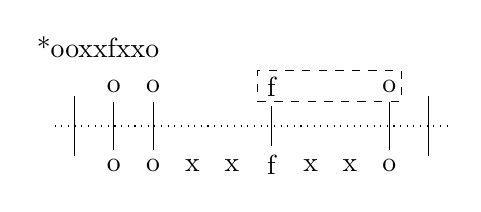
\begin{tikzpicture}
\node (1) at (0,0) {$\rtimes$};
\node (2) at (0.5,0) {o};
\node (3) at (1,0) {o};
\node (4) at (1.5,0) {x};
\node (5) at (2,0) {x};
\node (6) at (2.5,0) {f};
\node (7) at (3,0) {x};
\node (8) at (3.5,0) {x};
\node (9) at (4,0) {o};
\node (10) at (4.5,0) {$\ltimes$};
%
\node (01) at (0,1) {$\rtimes$};
\node (02) at (0.5,1) {o};
\node (03) at (1,1) {o};
\node (06) at (2.5,1) {f};
\node (09) at (4,1) {o};
\node (010) at (4.5,1) {$\ltimes$};
%
\foreach \Source/\Target in {%
	1.north/01.south,
	2.north/02.south,
	3.north/03.south,
	6.north/06.south,
	9.north/09.south,
	10.north/010.south%
    }
\draw (\Source) to (\Target);
%
\draw[dotted] (-0.25,0.5) to (4.8,0.5);
%
\node at (0.3,1.5) {*ooxxfxxo};
%
\draw [dashed] (2.33,0.81) -- (4.15,0.81) -- (4.15,1.21) -- (2.33,1.21) -- (2.33,0.81);
\end{tikzpicture}
\hspace{3em}
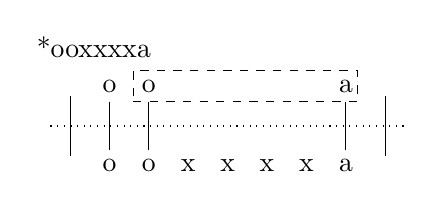
\begin{tikzpicture}
\node (1) at (0,0) {$\rtimes$};
\node (2) at (0.5,0) {o};
\node (3) at (1,0) {o};
\node (4) at (1.5,0) {x};
\node (5) at (2,0) {x};
\node (7) at (2.5,0) {x};
\node (8) at (3,0) {x};
\node (9) at (3.5,0) {a};
\node (10) at (4,0) {$\ltimes$};
%
\node (01) at (0,1) {$\rtimes$};
\node (02) at (0.5,1) {o};
\node (03) at (1,1) {o};
\node (09) at (3.5,1) {a};
\node (010) at (4,1) {$\ltimes$};
%
\foreach \Source/\Target in {%
	1.north/01.south,
	2.north/02.south,
	3.north/03.south,
	9.north/09.south,
	10.north/010.south%
    }
\draw (\Source) to (\Target);
%
\draw[dotted] (-0.25,0.5) to (4.3,0.5);
%
\node at (0.3,1.5) {*ooxxxxa};
%
\draw [dashed] (0.8,0.81) -- (3.65,0.81) -- (3.65,1.21) -- (0.8,1.21) -- (0.8,0.81);
\end{tikzpicture}
\end{center}
\caption{The extracted TSL grammar evaluating strings (Experiment $3$)}
\label{sgmnsge}
\end{figure}

\paragraph{Experiment 4: several vowel harmonies without blocking}

The learner induced that the ``consonant'' $x$ is not relevant for the vowel harmony system, and it also learned that on the tier of vowels, no disagreeing vowels can appear next to each other.
This learning outcome is therefore similar to the one of the second experiment, but with $4$ harmonic classes inferred instead of $2$.
This TSL grammar only generates words that are well-formed with respect to the rules of the vowel harmony  thus scoring $100$\% accuracy.

\begin{table}[h!]
\centering
\resizebox{\linewidth}{!}{%
\begin{tabular}{|r|l|}
\hline
\textbf{Pattern}            & \textit{several vowel harmonies, no blockers} \\ \hline
\textbf{Type of data}       & artificial data \\ \hline
\textbf{Example of data}    & xuuuxxxuuu, xxxeeexeee, xxxaaxxxaa, xoooxooxox, ... \\ \hline
%\textbf{Learned tier} & a, e, o, u  \\ \hline
\textbf{Learned $2$-TSL grammar} & (a, e, o, u)$_T$: ae, ao, ua, ue, uo, ... \\ \hline
\textbf{Generated sample}   & xxxaxaxaxax, xexxxexx, xxuxx, oxoxxox, ...\\ \hline
\textbf{Evaluation}         & \texttt{harmonic\_evaluator(sample, double\_harmony)} \\ \hline
\textbf{Score}              & $100$\%  \\ \hline
\end{tabular}}
\caption{TSL learning of several vowel harmonies without blockers; abstract representation.}
\end{table}


\paragraph{Experiment 5: several vowel harmonies with blocking}

The TSL learner correctly built a model for a Turkish-style harmonic system.
One tier is, indeed, able to capture both spreadings at the same time.
Given the tier consisting of all the vowels, the backness harmony can be expressed by a set of constraints of the type {[}$\alpha$front{]}{[}$-\alpha$front{]} (\emph{\"uu}, \emph{u\"u}, \emph{ae}, \emph{ea}, \emph{\"ua}, ...), and the rounding harmony that is blocked by non-high vowels is generalized as restrictions of the shape {[}$\alpha$round{]}{[}$-$high,$+$round{]} (\emph{oo}, \emph{uo}, \emph{eo}, ...) and {[}$\alpha$round{]}{[}$-\alpha$round, $+$high{]} (\emph{\"oi}, \emph{o\textsci}, \emph{au}, ...).
The performance of such model is $100$\%.

\begin{table}[h!]
\centering
\resizebox{\linewidth}{!}{%
\begin{tabular}{|r|l|}
\hline
\textbf{Pattern}            & \textit{several vowel harmonies with blockers} \\ \hline
\textbf{Type of data}       & artificial data \\ \hline
\textbf{Example of data}    & xx\"oexxix, xx\"u\"ux\"u\"ux, exxiixee, iiexxxex, xuuxxuuu, ... \\ \hline
%\textbf{Learned tier} & \textsci, \"o, \"u, a, e, i, o, u \\ \hline
\textbf{Learned $2$-TSL grammar} &  (\textsci, \"o, \"u, a, e, i, o, u)$_T$: \textsci\"o, \textsci\"u, \textsci e, \textsci i, \textsci o, ...\\ \hline
\textbf{Generated sample}   & xx\"oxxexx, x\textsci xxx, ax\textsci xxx, xaxxaxx, ...\\ \hline
\textbf{Evaluation}         & \texttt{harmonic\_evaluator(sample, backness\_and\_rounding)} \\ \hline
\textbf{Score}              & $100$\% overall ($100$\% backness only, $100$\% rounding only) \\ \hline
\end{tabular}
}
\caption{TSL learning of several harmonies with blockers; abstract representation.}
\end{table}

This result is theoretically expected since, in this pattern, there are two vowel harmonies happening at the same and affecting the same set of segments.
If we take two TSL grammars $G_1$ and $G_2$ that have the same tier alphabet but different sets of prohibited $n$-grams, taking a union of the prohibited $n$-grams would yield us another TSL grammar $G_3$.
Importantly, $G_3$ generates a language that is the intersection of the languages of $G_1$ and $G_2$.
To re-iterate this in more linguistic terms, \emph{two harmonies can fit on the same tier if the same sets of elements are involved in them}.




However, the learner did not perform well on the masked Turkish data.
It failed to remove $x$ from the tier since it did not observe \emph{\"o\"u} and \emph{ou} adjacent to each other, even though they are well-formed regarding the harmonic rules.
Its hypothesis, therefore, was not different from the one postulated by the SL grammar, and the accuracy of the model is $67$\%.

\begin{table}[h!]
\centering
\resizebox{\linewidth}{!}{%
\begin{tabular}{|r|l|}
\hline
\textbf{Pattern}            & \textit{several vowel harmonies with blockers} \\ \hline
\textbf{Type of data}       & masked Turkish data \\ \hline
\textbf{Example of data}    & xixxix, xuxx, xaaxa, xexxe, xax\textsci x, ... \\ \hline
%\textbf{Learned tier} & \textsci, \"o, \"u, a, e, i, o, u, x \\ \hline
\textbf{Learned $2$-TSL grammar} & (\textsci, \"o, \"u, a, e, i, o, u, x)$_T$: \textsci\"o, \textsci\"u, \textsci e, \textsci i, \textsci o, ...\\ \hline
\textbf{Generated sample}   & uux\"u\"ux, \"u, \textsci aaxeix, x\textsci\textsci\textsci\textsci x\"ue, ...\\ \hline
\textbf{Evaluation}         & \texttt{harmonic\_evaluator(sample, backness\_and\_rounding)} \\ \hline
\textbf{Score}              & $67$\% overall ($74$\% backness only, $74$\% rounding only) \\ \hline
\end{tabular}}
\caption{TSL learning of several harmonies with blockers; masked representation.}
\end{table}

The artificial dataset freely allowed vowel hiatus.
Harmonic vowels could be adjancent, such as in \emph{xxouxx}.
However, Turkish has gaps in what pairs of harmonic vowels can be adjacent in vowel hiatus.
Consequently, the performance of the TSL learner on the raw Turkish data was even worse, namely, $30$\%.



%The learner did not perform well on masked Turkish data, so, consequently, its performance was even worse on the raw data.
%Again, it failed to generalize the tier to a tier of vowels, and therefore was doing the same type of mistakes as the SL learner.
%Only $30$\% of the words predicted by the learned model were well-formed.



%
%\begin{table}[h!]
%\centering
%\begin{tabular}{|r|l|}
%\hline
%\textbf{Pattern}            & \textit{several vowel harmonies with blockers} \\ \hline
%\textbf{Type of data}       & raw Turkish data \\ \hline
%\textbf{Example of data}    & som, lafazan, konuk, kekti, lafzan, ... \\ \hline
%\textbf{Learned tier} & a, b, c, d, e, f, g, h, ... \\ \hline
%\textbf{Learned $2$-TSL grammar} & \u{g}o, \u{g}t, \u{g}v, \textsci\"o, \textsci\"u, ...\\ \hline
%\textbf{Generated sample}   & \"opoctal\textsci yov, sk, logsfig, eyu\c{c}m, ...\\ \hline
%\textbf{Evaluation}         & \texttt{harmonic\_evaluator(sample, backness\_and\_rounding)} \\ \hline
%\textbf{Score}              & $30$\% overall ($33$\% backness only, $35$\% rounding only) \\ \hline
%\end{tabular}
%\caption{TSL learning of several harmonies with blockers; raw representation}
%\end{table}


\subsection{Unsuccessful experiments}

TSL grammars can model patterns when a single set of elements is involved in a long-distance dependency.
However, if there is more than one long-distant process affecting different sets of elements, such as independent vowel and consonant harmonies, one tier is not enough.


\paragraph{Experiment 6: vowel harmony and consonant harmony without blocking}

It is impossible to model independent vowel and consonant harmonies using TSL grammars.
Vowels and consonants are involved in different long-distant phenomena, and therefore neither of them can be removed from the tier.
However, the presence of consonants does not allow us to represent vowels in a tier-based local fashion, and vice versa.
Therefore, neither vowel nor consonant harmony can be enforced: only $74$\% of the words generated by such grammar are well-formed.
This model is the same as its SL counterpart.

\begin{table}[h!]
\centering
\resizebox{\linewidth}{!}{%
\begin{tabular}{|r|l|}
\hline
\textbf{Pattern}            & \textit{vowel and consonant harmonies, no blockers} \\ \hline
\textbf{Type of data}       & artificial data \\ \hline
\textbf{Example of data}    & bbbaaabbaa, bbooboboob, pppoopppop, appaaappaa, ... \\ \hline
%\textbf{Learned tier} & a, b, o, p \\ \hline
\textbf{Learned $2$-TSL grammar} & (a, b, o, p)$_T$: ao, oa, bp, pb \\ \hline
\textbf{Generated sample}   & \textcolor{red!75!black}{apapoopop}, \textcolor{red!75!black}{oppoobbboopppob}, abab, \textcolor{red!75!black}{baaaap}, ...\\ \hline
\textbf{Evaluation}         & \texttt{harmonic\_evaluator(sample, double\_harmony\_no\_blockers)} \\ \hline
\textbf{Score}              & $74$\% \\ \hline
\end{tabular}}
\caption{TSL learning of vowel and consonant harmonies w/o blockers; abstract representation.}
\end{table}


\paragraph{Experiment 7: vowel harmony and consonant harmony with blocking}


Since TSL grammars failed to model the previous pattern with the independent vowel and consonant harmonies, they also fail to learn a similar pattern with a blocking effect.
Thus the performance of the TSL grammar, in this case, is again similar to its SL counterpart: $69$\%.


\begin{table}[h!]
\centering
\resizebox{\linewidth}{!}{%
\begin{tabular}{|r|l|}
\hline
\textbf{Pattern}            & \textit{vowel and consonant harmonies with blockers} \\ \hline
\textbf{Type of data}       & artificial data \\ \hline
\textbf{Example of data}    & pppoootopt, obbbtpooot, aabbbaatat, pppaapappp, ... \\ \hline
%\textbf{Learned tier} & a, b, o, p, t \\ \hline
\textbf{Learned $2$-TSL grammar} & (a, b, o, p, t)$_T$: ao, oa, bp, pb, tb \\ \hline
\textbf{Generated sample}   & \textcolor{red!75!black}{ptopaba}, btoptttpt, a, pppa, ob, ... \\ \hline
\textbf{Evaluation}         & \texttt{harmonic\_evaluator(sample, double\_harmony\_with\_blockers)} \\ \hline
\textbf{Score}              & $69$\% \\ \hline
\end{tabular}}
\caption{TSL learning of vowel and consonant harmonies with blockers; abstract representation.}
\end{table}


\paragraph{Experiment 8: unbounded tone plateauing}

There is no choice of a tier alphabet that would allow a TSL grammar to capture the \emph{no H...L...H} generalization.
If $H$ and $L$ are both present on the tier, such TSL grammar behaves like the SL one.
Otherwise either $H$ or $L$ needs to be omitted from the tier, but both of them are crucially important for the generalization.
Hence the pattern of UTP is neither SL nor TSL.
The learned grammar performs with the accuracy of $90$\% exclusively due to a small alphabet and the majority of the generated strings being short.

\begin{table}[h!]
\centering
\resizebox{\linewidth}{!}{%
\begin{tabular}{|r|l|}
\hline
\textbf{Pattern}            & \textit{unbounded tone plateauing} \\ \hline
\textbf{Type of data}       & artificial data \\ \hline
\textbf{Example of data}    & HHHHH, LHHLL, LHHHH, LHHHH, HHHHH, ... \\ \hline
%\textbf{Learned tier} & H, L \\ \hline
\textbf{Learned $3$-TSL grammar} & (H, L)$_T$: HLH \\ \hline
\textbf{Generated sample}   & \textcolor{red!75!black}{HHHLLH}, HLL, \textcolor{red!75!black}{HHLLHHLLLHLLLLLHHL}, LLLLH, ... \\ \hline
\textbf{Evaluation}         & \texttt{evaluate\_utp\_strings(sample)} \\ \hline
\textbf{Score}              & $90$\% \\ \hline
\end{tabular}}
\caption{TSL learning of unbounded tone plateauing; abstract representation.}
\end{table}


\paragraph{Experiment 9: first-last harmony}

As expected, the TSL learner cannot learn the unattested pattern of the first-last harmony.
In fact, the obtained grammar is the same as the one proposed by the SL learner, and therefore it makes exactly the same types of mistakes.

\begin{table}[h!]
\centering
\resizebox{\linewidth}{!}{%
\begin{tabular}{|r|l|}
\hline
\textbf{Pattern}            & \textit{first-last harmony} \\ \hline
\textbf{Type of data}       & artificial data \\ \hline
\textbf{Example of data}    & axoaaxaxaa, aaxaaxxxoa, ooaxaoaooo, axxoaxaaaa, ... \\ \hline
%\textbf{Learned tier} & a, o, x \\ \hline
\textbf{Learned $2$-TSL grammar} & (a, o, x)$_T$: \bow x, x\eow \\ \hline
\textbf{Generated sample}   & \textcolor{red!75!black}{aaoxaxxoxao}, aaxaooxa, \textcolor{red!75!black}{axooaao}, oxxo, ... \\ \hline
\textbf{Evaluation}         & \texttt{evaluate\_first\_last\_words(sample)} \\ \hline
\textbf{Score}              & $50$\% \\ \hline
\end{tabular}}
\caption{TSL learning of first-last harmony; abstract representation.}
\end{table}



\subsection{TSL experiments: interim summary}

A TSL learner, if given a representative sample of data, extracts a \emph{tier alphabet} that represents a set of elements involved in a long-distance dependency.
If every item of that set is also involved in another dependency, it can capture such cases as well, as it did in case of the abstract pattern of Turkish harmony.
Overall, TSL learner succeeded in building a grammar for every pattern that exhibited either a local dependency or a long-distance dependency among a single set of elements if given a representative sample.

However, if there is more than a single set of items involved in different long-distance dependencies, this cannot be modeled by TSL grammars.
Therefore TSL learner failed on a challenge that included learning separate vowel and consonant harmonies: for those cases, one tier is not enough.


\section{Multi-tier strictly local models}

Previous two sections explore two different perspectives on modeling long-distance dependencies.
Strictly piecewise grammars prohibit subsequences elements of which can be \emph{arbitrarily far} from each other.
SP models thus handle cases of multiple long-distance dependencies; however, none of them can include blockers.
Also, SP models can \emph{only} model long-distance dependencies: they cannot handle locally bounded patterns.
TSL grammars can encode local patterns and also blocking effects; however, they are limited to a \emph{single} set of items involved in a long-distance dependency.
Hence they cannot encode such cases as independent vowel and consonant harmonies within the same language.
In this section, I explore the performance of multi-tier strictly local (MTSL) models: namely, models that employ several TSL grammars at the same time.



\subsection{MTSL learning algorithm}
\label{mtsllearner}

The subregular class of MTSL grammars is a proper extension of TSL.
However, the $k$TSLIA algorithm introduced earlier cannot be simply extended from a single tier to multiple ones since its initial assumption is that \emph{all members of $\Sigma$} belong to a tier alphabet: it implicitly assumes the existence of just a single tier.

Together with Kevin McMullin and Aniello De Santo, we developed the MTSL learning algorithm \emph{MTSL$2$IA} \citep{McMullinAksenovaDeSanto2019}.
While there are several approaches to learning SL, SP, and TSL languages, MTSL$2$IA is the first published algorithm that tackles the problem of extracting MTSL grammars.
It relies on the assumption that we can first detect all the prohibited $k$-grams, and then learn a tier for every one of them .
Thus, we learn \emph{a tier for every negative bigram} of the MTSL grammar.
Currently, this algorithm only works with $2$-local restrictions, and the work of extending it to $k$ is ongoing.

Crucially, the MTSL$2$IA algorithm relies on the notion of a \emph{path} denoted as $\langle\rho_1, X, \rho_2\rangle$.
It can be thought of as a subsequence $(\rho_1\dots\rho_2)$ accompanied by a set of symbols $X$ that occurred in-between $\rho_1$ and $\rho_2$ in the training sample. For example, the following paths can be extracted from a string \emph{abac}:
$\langle a, \{\}, b \rangle$,
$\langle a, \{b\}, a \rangle$,
$\langle a, \{b, a\}, c \rangle$,
$\langle b, \{\}, a \rangle$,
$\langle b, \{a\}, c \rangle$, and 
$\langle b, \{\}, c \rangle$.


\begin{algorithm}[h!]
\caption{Extracts $G_{MTSL_{2}}$ from $I$}
\begin{algorithmic}
\REQUIRE a finite input sample $I \in \Sigma^*$
\STATE $B \leftarrow~ \Sigma^2 \cap \textrm{ngram}(I, 2)$
\STATE $i \leftarrow~ 1$
\FOR {$\rho_1\rho_2 \in~ B$}
	\STATE $R_i \leftarrow~ \rho_1\rho_2$
	\STATE $T_i \leftarrow~ \Sigma$
	\FOR {$\sigma \in~ \Sigma \cap \{\rho_1, \rho_2\}$}
		\IF {$\forall \langle\rho_1, X, \rho_2\rangle \in \textrm{path}(I) \textrm{ s.t. } \sigma\in~X, \langle\rho_1, X - \{\sigma\}, \rho_2\rangle~ \in \textrm{path}(I)$}
			\STATE $T_i \leftarrow~ T_i - \{\sigma\}$
		\ENDIF
	\ENDFOR
	\STATE $G_i \leftarrow~ \langle~ T_i, R_i \rangle$
	\STATE $i \leftarrow~ i+1$
\ENDFOR
\STATE $G \leftarrow~ G_1 \wedge G_2 \dots G_{\mid B\mid -1} \wedge G_{\mid B\mid}$
\RETURN $G$
\end{algorithmic}
\end{algorithm}

\textbf{Intuitively}, this algorithm works as follows.
At first, it detects a list of bigrams $B$ that is unattested in the training sample $I$.
Then it loops over all elements of $B$, and for every bigram $\rho_1\rho_2 \in~ B$, it assumes that the tier for that bigram is $\Sigma$.
Afterwards it collects a set of all paths of the form $\langle\rho_1, X, \rho_2\rangle$, and finds all symbols $\sigma \in~ \Sigma$ that can be removed from $X$ so that the newly obtained path $\langle\rho_1, X\setminus\{\sigma\}, \rho_2\rangle$ is still attested in the list of paths of $I$.
It then removes such $\sigma$ from a tier associated with $\rho_1\rho_2$.
After all members of $B$ were processed, the algorithm outputs a grammar $G$ that is a collection of all unattested bigrams with the tiers corresponding to those bigrams; see the \textbf{pseudocode} above.
Similarly to the learners discussed in the previous subsections, MTSL$2$IA learns the grammar from a positive sample in polynomial time and data \citep{McMullinAksenovaDeSanto2019}.

\paragraph{Example}
Imagine having a dataset that exhibits long-distance sibilant assimilation between \emph{\textesh} and \emph{s} unless blocked by \emph{f}.
Additionally, it also has vowel harmony affecting \emph{a} and \emph{o}.
This dataset includes the following strings: \emph{saasa, \textesh a\textesh aa, sooos, o\textesh o\textesh o, \textesh ofos, \textesh afas, sofo\textesh, safa\textesh, sf\textesh, sf\textesh,} and so on.
Of course, strings violating the rules of sibilant (such as \emph{\textesh aa\textesh as} or \emph{so\textesh ooa}) or vowel (\emph{a\textesh oo}, \emph{sosoa}) harmony are not included in the training sample.
As soon as the sample is given as input to the learner, the learner notices the absence of bigrams \emph{s\textesh , \textesh s, ao} and \emph{oa}.
When it explores the bigram \emph{s\textesh}, one of the paths to consider is $\langle s, \{a\}, \textrm{\textesh}\rangle$.
However, $\langle s, \{\}, \textrm{\textesh}\rangle$ is also a valid path, so \emph{a} is not a tier element for the bigram \emph{s\textesh}, and neither is \emph{o}.
When the unattested bigram \emph{ao} is explored, the learner does not detect any paths that would involve the symbols \{$s$, \textesh, $f$\}.
The condition of the if-statement is then trivially satisfied, and therefore \emph{s, \textesh} and \emph{f} are removed from the tier of that bigram.
A concise representation of the grammar that the learner induced is the following:

\begin{itemize}
	\item $G_1 = \langle T_1 = \{a, o\}, R_1 = \{ao, oa\}\rangle$;
	\item $G_2 = \langle T_2 = \{s, \textrm{\textesh}, f\}, R_2 = \{\textrm{\textesh}s, s\textrm{\textesh}\}\rangle$.
\end{itemize}

However, the \emph{tier-per-bigram} assumption comes with a caveat.
It results in the algorithm failing to capture patterns where the same bigram is present on several different tiers.
For example, consider an MTSL grammar where the bigram \emph{xx} is prohibited on two tiers: $T_1 = \{x, a\}$ and $T_2 = \{x, b\}$.
Instead, the MTSL$2$IA learner would converge on the incorrect tier $T = \{x, a, b\}$.
Tier configurations that cannot be learned by this learner is a sub-case of a general case when two tier alphabets have a non-empty intersection that does not overlap with either of the alphabets.
Interestingly, we show in \citet{AksenovaDeshmukh2018} that in natural languages, if two agreements require two different tiers, those tiers never overlap unless one of them is properly contained within the other one.
Therefore if applied to phonological data, this learner could be more efficient in comparison to the learner that would also explore the typologically unattested class of tier configurations.

As noted previously, this algorithm learns $2$-local MTSL grammars, but we are currently working on extending it to arbitrary $k$.
Intuitively, this can be done by extending the notion of a path.
Its shape could be generalized as $\langle\rho_1, X_1, \rho_2, X_2, \dots \rho_{n-1}, X_{n-1}, \rho_n\rangle$, where $\rho_1\rho_2\dots\rho_n$ is a $k$-long sequence, and $X_i$ is the set of symbols that occurred in-between $\rho_i$ and $\rho_{i+1}$ in the training sample.
The condition of the if-statement needs to also be adjusted to accommodate for longer paths; but otherwise, the logic of the algorithm stays the same.



\subsection{Successful experiments}

In this subsection, I show that MTSL grammars can be used to successfully model all of the discussed types of local and long-distant dependencies.
Even when challenged with the raw data of German, Finnish, and Turkish, the MTSL learner extracts the corresponding MTSL grammars with the impressive accuracies of $100$\%, $100$\%, and $95$\%, correspondingly.
The patterns of unbounded tone plateauing and the first-last harmony are not MTSL in their nature, and therefore cannot be learned using the MTSL inference algorithm.


\paragraph{Experiment 1: word-final devoicing}

Since MTSL grammars are a proper superclass of TSL grammars, and, consequently, of the SL ones, the MTSL learning algorithm acquires the pattern of word-final devoicing.
The performance of the MTSL model on the raw German dataset is $100$\%, as well as on the other representations of that pattern.

\begin{table}[h!]
\centering
\resizebox{\linewidth}{!}{%
\begin{tabular}{|r|l|}
\hline
\textbf{Pattern}            & \textit{word-final devoicing}  \\ \hline
\textbf{Type of data}       & raw German data \\ \hline
\textbf{Example of data}    & hochjagende, zugebliebener, verbricht, besuchszimmer, ... \\ \hline
\textbf{Learned $2$-MTSL grammar} & \emph{too large: $294$ tiers!} \\ \hline
\textbf{Generated sample}   & mugoftkuh\"ampo, kisizkkokg\"up, rk\"ums\"ubtal... \\ \hline
\textbf{Evaluation}         & \texttt{evaluate\_wfd\_words(sample)}   \\ \hline
\textbf{Score}              & $100$\%   \\ \hline
\end{tabular}}
\caption{MTSL learning of the word-final devoicing; raw representation.}
\end{table}


%
%\begin{table}[h!]
%\centering
%\begin{tabular}{|r|l|}
%\hline
%\textbf{Pattern}            & \textit{word-final devoicing} \\ \hline
%\textbf{Type of data}       & artificial data  \\ \hline
%\textbf{Example of data}    & aaabbpbbbp, pbapbapapa, apabaappap, bbbbaabbbp, ... \\ \hline
%\textbf{Learned $2$-MTSL grammar} & (a, b, p)$_T$: b\eow, \bow\eow  \\ \hline
%\textbf{Generated sample}   & pp, pbpapaba, bpppp, aap, bp, ...  \\ \hline
%\textbf{Evaluation}         & \texttt{evaluate\_wfd\_words(sample)} \\ \hline
%\textbf{Score}              & $100$\% \\ \hline
%\end{tabular}
%\caption{MTSL learning of the word-final devoicing; abstract representation}
%\end{table}

%\begin{table}[h!]
%\centering
%\begin{tabular}{|r|l|}
%\hline
%\textbf{Pattern}            & \textit{word-final devoicing}    \\ \hline
%\textbf{Type of data}       & masked German data \\ \hline
%\textbf{Example of data}    & aakaabaaaa, aakaabaaak, aakaa, aakat, aaa, ... \\ \hline
%\textbf{Learned $2$-MTSL grammar} & (a, b, d, g, k, p, t)$_T$: b\eow, d\eow, g\eow, \bow\eow              \\ \hline
%\textbf{Generated sample}   & agdgdbgkdapk, dptkp, pktbdkgtadpa, tgdgp, ... \\ \hline
%\textbf{Evaluation}         & \texttt{evaluate\_wfd\_words(sample)} \\ \hline
%\textbf{Score}              & $100$\%  \\ \hline
%\end{tabular}
%\caption{MTSL learning of the word-final devoicing; masked representation}
%\end{table}




\paragraph{Experiment 2: a single vowel harmony without blocking}

Similarly, the MTSL learner extracted the grammar representing a single vowel harmony pattern without a blocking effect.
The learner induced a single tier containing symbols $a$ and $o$.
The grammar for this tier was the same one as in the TSL version of this experiment: $ao$, $oa$.
$100$\% of the words generated by the obtained grammar were well-formed.
The success of the MTSL learner on this and further experiments where the TSL learner performed well follows from the fact that the class of MTSL languages subsumes TSL languages. 


\begin{table}[h!]
\centering
\resizebox{\linewidth}{!}{%
\begin{tabular}{|r|l|}
\hline
\textbf{Pattern}            & \textit{one vowel harmony, no blockers} \\ \hline
\textbf{Type of data}       & artificial data \\ \hline
\textbf{Example of data}    & oxxxooxxxx, ooxxxooxxo, aaxxxaaxxx, oxxxxoxxxo, ... \\ \hline
\textbf{Learned $2$-MTSL grammar} & (a, o)$_T$: ao, oa \\ \hline
\textbf{Generated sample}   & xxoox, xxaxaxa, axaaax, xooox, ... \\ \hline
\textbf{Evaluation}         & \texttt{harmonic\_evaluator(sample, single\_harmony\_no\_blockers)}  \\ \hline
\textbf{Score}              & $100$\%   \\ \hline
\end{tabular}}
\caption{MTSL learning of a single harmony without blockers; abstract representation.}
\end{table}

%\begin{table}[h!]
%\centering
%\begin{tabular}{|r|l|}
%\hline
%\textbf{Pattern}            & \textit{one vowel harmony, no blockers}  \\ \hline
%\textbf{Type of data}       & masked Finnish data \\ \hline
%\textbf{Example of data}    & xaxxixxex, xix\"axixex, xaxxixxaxix, uxxuxaxxix, ... \\ \hline
%\textbf{Learned $2$-MTSL grammar} & \begin{tabular}[c]{@{}l@{}}
%(u, y)$_T$: yu, uy; 
%(\"a, u)$_T$: \"au, u\"a; 
%(\"o, o)$_T$: \"oo, o\"o; etc.
%\end{tabular} \\ \hline
%\textbf{Generated sample}   & \"oyxy\"a\"o\"oyyy\"o, \"oyxy\"a\"o, \"ayx, oxxuxaxu, ... \\ \hline
%\textbf{Evaluation}         & \texttt{harmonic\_evaluator(sample, front\_harmony)}   \\ \hline
%\textbf{Score}              & $100$\%  \\ \hline
%\end{tabular}
%\caption{MTSL learning of a single harmony without blockers; masked representation}
%\end{table}

The MTSL inference algorithm also successfully learned the generalization from raw and masked Finnish datasets.
Indeed, $100$\% of the words generated by the grammar, such as \emph{rjegovnj} or \emph{l\"ay\"omppl}, are harmonic.
Although the grammar is transparent and fully interpretable, it postulates $266$ tiers.
An open question is to explain \emph{how exactly} increasing the number of tiers helped the learner to tackle this challenge.


\begin{table}[h!]
\centering
\resizebox{\linewidth}{!}{%
\begin{tabular}{|r|l|}
\hline
\textbf{Pattern}            & \textit{one vowel harmony, no blockers}  \\ \hline
\textbf{Type of data}       & raw Finnish data \\ \hline
\textbf{Example of data}    & mathilden, lis\"animen, macmillanin, urquhartin, ... \\ \hline
\textbf{Learned $2$-MTSL grammar} & \emph{too large: $266$ tiers!} \\ \hline
\textbf{Generated sample}   & rjegovnj, l\"ay\"omppl, axiflt, sil\"o\"a\"amydv, ... \\ \hline
\textbf{Evaluation}         & \texttt{harmonic\_evaluator(sample, front\_harmony)} \\ \hline
\textbf{Score}              & $100$\%  \\ \hline
\end{tabular}}
\caption{MTSL learning of a single harmony without blockers; raw representation.}
\end{table}



\paragraph{Experiment 3: a single vowel harmony with blocking}

Again, the success of the MTSL learner in this experiment follows from the fact that TSL grammars are a proper subset of the MTSL ones.
However, what is surprising is that the MTSL inference algorithm did not converge on a single tier: instead, it postulated $3$ different tiers.

The learner discovered $3$ unattested bigrams: $ao$, $fo$, and $oa$.
However, in none of the data points $a$ was ever followed by $o$, so there were no paths of the type $\langle a, X, o\rangle$: trivially, elements $f$ and $x$ were considered irrelevant for this restriction.
Similarly, $a$ was excluded from a tier induced for the restriction $fo$ because $f$ is never followed by $o$.
But when considering the unattested bigram $oa$, paths such as $\langle o, \{f\}, a\rangle$ and $\langle o, \{f, x\}, a\rangle$ were found in the data, while the ones such as $\langle o, \{\}, a\rangle$ were not.
A symbol $x$ was hence removed from the tier of the bigram $oa$, but the blocker $f$ was not.
In such a way, MTSL learner constructs $3$ different tiers, but the language of the obtained grammar is equivalent to the one of the TSL grammar $\{oa, ao, fo\}$ with the tier $T = \{a, o, f\}$.

\begin{table}[h!]
\centering
\resizebox{\linewidth}{!}{%
\begin{tabular}{|r|l|}
\hline
\textbf{Pattern}            & \textit{one vowel harmony with blockers} \\ \hline
\textbf{Type of data}       & artificial data \\ \hline
\textbf{Example of data}    & oxxxooxxxx, xxooxfaaax, aaxxxaaxxx, ofxxafxxaa, ... \\ \hline
\textbf{Learned $2$-MTSL grammar} & \begin{tabular}[c]{@{}l@{}}
(a, o)$_T$: ao; 
(f, o)$_T$: fo; 
(a, f, o)$_T$: oa.
\end{tabular} \\ \hline
\textbf{Generated sample}   & oxffxax, faaaxffa, ofxaaf, fa, ooooof, ...\\ \hline
\textbf{Evaluation}         & \texttt{harmonic\_evaluator(sample, single\_harmony\_with\_blockers)}    \\ \hline
\textbf{Score}              & $100$\%  \\ \hline
\end{tabular}}
\caption{MTSL learning of a single harmony with blockers; abstract representation.}
\end{table}


\paragraph{Experiment 4: several vowel harmonies without blocking}

This experiment was successful since the MTSL learner extracted the grammar for the pattern of several vowel harmonies without a blocking effect.
However, similarly to the previous example, the resulting grammar was not the same as the one extracted by the TSL learner.
The MTSL algorithm constructed a separate tier for every pair of the potentially disagreeing elements, while correctly noticing that the transparent element $x$ is irrelevant for the generalization.

\begin{table}[h!]
\centering
\resizebox{\linewidth}{!}{%
\begin{tabular}{|r|l|}
\hline
\textbf{Pattern}            & \textit{several vowel harmonies, no blockers} \\ \hline
\textbf{Type of data}       & artificial data \\ \hline
\textbf{Example of data}    & xuuuxxxuuu, xxxeeexeee, xxxaaxxxaa, xoooxooxox, ... \\ \hline
\textbf{Learned $2$-MTSL grammar} & \begin{tabular}[c]{@{}l@{}}
(u, o)$_T$: uo, ou; 
(a, u)$_T$: au, ua; 
(o, e)$_T$: eo, oe; etc.
\end{tabular} \\ \hline
\textbf{Generated sample}   & xuxuuuxu, xoox, aaa, exexxe ...\\ \hline
\textbf{Evaluation}         & \texttt{harmonic\_evaluator(sample, double\_harmony)} \\ \hline
\textbf{Score}              & $100$\%  \\ \hline
\end{tabular}}
\caption{MTSL learning of several vowel harmonies without blockers; abstract representation.}
\end{table}



\paragraph{Experiment 5: several vowel harmonies with blocking}

The MTSL induction algorithm found a way to model several vowel harmonies with a blocking effect.
Also, similarly to the examples discussed above, more than a single tier was inferred.
All of the words generated by the extracted MTSL grammar were well-formed regarding the rules of Turkish harmony.

\begin{table}[h!]
\centering
\resizebox{\linewidth}{!}{%
\begin{tabular}{|r|l|}
\hline
\textbf{Pattern}            & \textit{several vowel harmonies with blockers} \\ \hline
\textbf{Type of data}       & artificial data \\ \hline
\textbf{Example of data}    & xx\"oexxix, xx\"u\"ux\"u\"ux, exxiixee, iiexxxex, xuuxxuuu, ... \\ \hline
\textbf{Learned $2$-MTSL grammar} & \begin{tabular}[c]{@{}l@{}}
(\"u, e, i)$_T$: \"ui; 
(\"u, e)$_T$: e\"u; 
(\textsci, \"o)$_T$: \textsci\"o, \"o\textsci; etc.
\end{tabular} \\ \hline
\textbf{Generated sample}   & \textsci xxaaaa, \"uexi, \"uxeexe, \"o\"u\"u\"ue, \"o\"uexe, ... \\ \hline
\textbf{Evaluation}         & \texttt{harmonic\_evaluator(sample, backness\_and\_rounding)} \\ \hline
\textbf{Score}              & $100$\% overall ($100$\% backness only, $100$\% rounding only) \\ \hline
\end{tabular}}
\caption{MTSL learning of several harmonies with blockers; abstract representation.}
\end{table}


Some of the configurations that the MTSL learner was looking for were missing in the masked and raw representations of the Turkish data, and therefore the accuracies of those models were slightly worse than ideal: both of them scored $95$\%.
As of the MTSL grammar inferred from the raw data, it relies on $266$ tiers, and the way it is able to perform so well is worth further investigation.

%\begin{table}[h!]
%\centering
%\begin{tabular}{|r|l|}
%\hline
%\textbf{Pattern}            & \textit{several vowel harmonies with blockers} \\ \hline
%\textbf{Type of data}       & masked Turkish data \\ \hline
%\textbf{Example of data}    & xixxix, xuxx, xaaxa, xexxe, xax\textsci x, ... \\ \hline
%\textbf{Learned $2$-MTSL grammar} & \begin{tabular}[c]{@{}l@{}}
%(\"u, e, i, x)$_T$: \"ui; 
%(\"u, o, x)$_T$: \"o\"u; 
%(\"u, e)$_T$: \"ue; etc.
%\end{tabular} \\ \hline
%\textbf{Generated sample}   & \"uxxeeee, xox\textsci a\textsci, exxxeixixei, ux\textsci xxa, ...\\ \hline
%\textbf{Evaluation}         & \texttt{harmonic\_evaluator(sample, backness\_and\_rounding)} \\ \hline
%\textbf{Score}              & $95$\% overall ($100$\% backness only, $95$\% rounding only) \\ \hline
%\end{tabular}
%\caption{MTSL learning of several harmonies with blockers; masked representation}
%\end{table}

\begin{table}[h!]
\centering
\resizebox{\linewidth}{!}{%
\begin{tabular}{|r|l|}
\hline
\textbf{Pattern}            & \textit{several vowel harmonies with blockers} \\ \hline
\textbf{Type of data}       & raw Turkish data \\ \hline
\textbf{Example of data}    & som, lafazan, konuk, kekti, lafzan, ... \\ \hline
\textbf{Learned $2$-MTSL grammar} &  \emph{too large: $266$ tiers!} \\ \hline
\textbf{Generated sample}   & apn\textsci c\textsci r\textsci saa,  tel\c{c}it\c{c}eeriden, mbezkdenic, ...\\ \hline
\textbf{Evaluation}         & \texttt{harmonic\_evaluator(sample, backness\_and\_rounding)} \\ \hline
\textbf{Score}              & $95$\% overall ($100$\% backness only, $95$\% rounding only) \\ \hline
\end{tabular}}
\caption{MTSL learning of several harmonies with blockers; raw representation.}
\end{table}


\paragraph{Experiment 6: vowel harmony and consonant harmony without blocking}

The pattern of independent vowel and consonant harmonies can be captured using two tiers: one for vowels, and another one for consonants.
The tier of vowels prohibits $oa$ and $ao$, and the tier of consonants rules out $pb$ and $bp$.
To evaluate the well-formedness of a word, both of its tiers need to be inspected individually.
For example, consider a word \emph{ababbabb}.
Tts consonant tier contains \emph{bbbbb}, and the vowel tier is \emph{aaa}: both of them are well-formed.
However, words such as \emph{ababbbob} are not grammatical: even though the consonant tier does not contain violations, the vowel tier is \emph{a\textbf{ao}}, and it violates the rules of the vowel harmony.
The language of this MTSL grammar is the intersection of two TSL grammars, one per every harmony.
The accuracy of this model is $100$\%.

\begin{table}[h!]
\centering
\resizebox{\linewidth}{!}{%
\begin{tabular}{|r|l|}
\hline
\textbf{Pattern}            & \textit{vowel and consonant harmonies, no blockers} \\ \hline
\textbf{Type of data}       & artificial data \\ \hline
\textbf{Example of data}    & bbbaaabbaa, bbooboboob, pppoopppop, appaaappaa, ... \\ \hline
\textbf{Learned $2$-MTSL grammar} & \begin{tabular}[c]{@{}l@{}}
(a, o)$_T$: ao, oa; 
(b, p)$_T$: pb, bp.
\end{tabular} \\ \hline
\textbf{Generated sample}   & oapapaaa, obbb, babbba, poop, ...\\ \hline
\textbf{Evaluation}         & \texttt{harmonic\_evaluator(sample, double\_harmony\_no\_blockers)} \\ \hline
\textbf{Score}              & $100$\% \\ \hline
\end{tabular}}
\caption{MTSL learning of vowel and consonant harmonies w/o blockers; abstract representation.}
\end{table}


\paragraph{Experiment 7: vowel harmony and consonant harmony with blocking}

MTSL learner performs $100$\% accurate on the pattern with vowel and consonant harmonies even if they include blockers, and it is the only subregular model among the discussed ones that is able to do so.
In this case, the learner extracts $4$ tiers, and a total of $5$ prohibited bigrams.
The choice of the tiers can be explained in the same way it was done for the third experiment.
On the tier of vowels, the grammar prohibits their disagreeing combinations $ao$ and $oa$.
The consonant-related restrictions are located across $3$ different tiers due to the inference steps of the algorithm, but these restrictions, in fact, can be expressed on a single tier containing $p$, $b$, and $t$.
Figure \ref{fakjfanfk} shows the MTSL evaluation of strings \emph{aabbotoob} and \emph{aabbaaaap} using a simplified yet equivalent MTSL grammar containing only $2$ tiers: one for vowels, and another for consonants.

\begin{table}[h!]
\centering
\resizebox{\linewidth}{!}{%
\begin{tabular}{|r|l|}
\hline
\textbf{Pattern}            & \textit{vowel and consonant harmonies with blockers} \\ \hline
\textbf{Type of data}       & artificial data \\ \hline
\textbf{Example of data}    & pppoootopt, obbbtpooot, aabbbaatat, pppaapappp, ... \\ \hline
\textbf{Learned $2$-MTSL grammar} & \begin{tabular}[c]{@{}l@{}}
(b, p, t)$_T$: bp; 
(a, o)$_T$: ao, oa;
(b, p)$_T$: pb;
(b, t)$_T$: tb.
\end{tabular} \\ \hline
\textbf{Generated sample}   & obtppoppo, totoo, ap, ooptpp, abtatat, ... \\ \hline
\textbf{Evaluation}         & \texttt{harmonic\_evaluator(sample, double\_harmony\_with\_blockers)} \\ \hline
\textbf{Score}              & $100$\% \\ \hline
\end{tabular}}
\caption{MTSL learning of vowel and consonant harmonies with blockers; abstract representation.}
\end{table}

\begin{figure}[h!]
\begin{center}
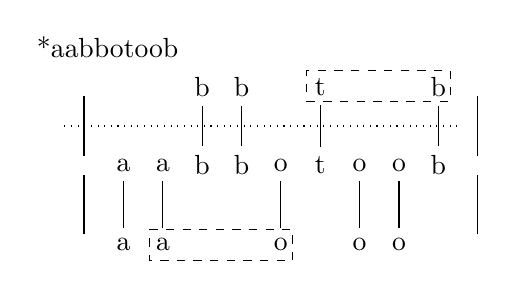
\begin{tikzpicture}
\node (1) at (0,0) {$\rtimes$};
\node (2) at (0.5,0) {a};
\node (3) at (1,0) {a};
\node (4) at (1.5,0) {b};
\node (5) at (2,0) {b};
\node (6) at (2.5,0) {o};
\node (7) at (3,0) {t};
\node (8) at (3.5,0) {o};
\node (9) at (4,0) {o};
\node (10) at (4.5,0) {b};
\node (11) at (5,0) {$\ltimes$};
%
\node (001) at (0,-1) {$\rtimes$};
\node (002) at (0.5,-1) {a};
\node (003) at (1,-1) {a};
\node (006) at (2.5,-1) {o};
\node (008) at (3.5,-1) {o};
\node (009) at (4,-1) {o};
\node (0011) at (5,-1) {$\ltimes$};
%
\node (01) at (0,1) {$\rtimes$};
\node (04) at (1.5,1) {b};
\node (05) at (2,1) {b};
\node (07) at (3,1) {t};
\node (010) at (4.5,1) {b};
\node (011) at (5,1) {$\ltimes$};
%
\foreach \Source/\Target in {%
	1.north/01.south,
	4.north/04.south,
	5.north/05.south,
	7.north/07.south,
	11.north/011.south,
	10.north/010.south%
    }
\draw (\Source) to (\Target);
%
\foreach \Source/\Target in {%
	001.north/1.south,
	002.north/2.south,
	003.north/3.south,
	006.north/6.south,
	008.north/8.south,
	009.north/9.south,
	0011.north/11.south%
    }
\draw (\Source) to (\Target);
%
\draw[dotted] (-0.25,0.5) to (4.8,0.5);
%
\node at (0.3,1.5) {*aabbotoob};
%
\draw [dashed] (2.83,0.81) -- (4.65,0.81) -- (4.65,1.21) -- (2.83,1.21) -- (2.83,0.81);
\draw [dashed] (0.83,-0.81) -- (2.65,-0.81) -- (2.65,-1.21) -- (0.83,-1.21) -- (0.83,-0.81);
\end{tikzpicture}
\hspace{3em}
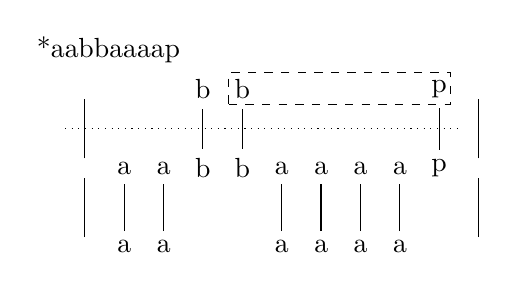
\begin{tikzpicture}
\node (1) at (0,0) {$\rtimes$};
\node (2) at (0.5,0) {a};
\node (3) at (1,0) {a};
\node (4) at (1.5,0) {b};
\node (5) at (2,0) {b};
\node (6) at (2.5,0) {a};
\node (7) at (3,0) {a};
\node (8) at (3.5,0) {a};
\node (9) at (4,0) {a};
\node (10) at (4.5,0) {p};
\node (11) at (5,0) {$\ltimes$};
%
\node (001) at (0,-1) {$\rtimes$};
\node (002) at (0.5,-1) {a};
\node (003) at (1,-1) {a};
\node (006) at (2.5,-1) {a};
\node (007) at (3,-1) {a};
\node (008) at (3.5,-1) {a};
\node (009) at (4,-1) {a};
\node (0011) at (5,-1) {$\ltimes$};
%
\node (01) at (0,1) {$\rtimes$};
\node (04) at (1.5,1) {b};
\node (05) at (2,1) {b};
\node (010) at (4.5,1) {p};
\node (011) at (5,1) {$\ltimes$};
%
\foreach \Source/\Target in {%
	1.north/01.south,
	4.north/04.south,
	5.north/05.south,
	11.north/011.south,
	10.north/010.south%
    }
\draw (\Source) to (\Target);
%
\foreach \Source/\Target in {%
	001.north/1.south,
	002.north/2.south,
	003.north/3.south,
	006.north/6.south,
	007.north/7.south,
	008.north/8.south,
	009.north/9.south,
	0011.north/11.south%
    }
\draw (\Source) to (\Target);
%
\draw[dotted] (-0.25,0.5) to (4.8,0.5);
%
\node at (0.3,1.5) {*aabbaaaap};
%
\draw [dashed] (1.83,0.81) -- (4.65,0.81) -- (4.65,1.21) -- (1.83,1.21) -- (1.83,0.81);
\end{tikzpicture}
\end{center}
\caption{Experiment $7$: the extracted MTSL grammar evaluating the ungrammatical strings \emph{aabbotoob} and \emph{aabbaaaap}.}
\label{fakjfanfk}
\end{figure}



\subsection{Unsuccessful experiments}

I was not able to test the performance of the MTSL learner on the UTP pattern since this learner currently exists only for $2$-local dependencies, and UTP requires postulating a $3$-local restriction.
However, this pattern is not MTSL expressible since there is no tier or a combination of tiers that would be able to express that generalization.
Hence the only unsuccessful experiment that I present in this subsection is the expected inability of MTSL grammars to express the first-last harmony.


\paragraph{Experiment 9: first-last harmony}

MTSL grammars cannot encode the pattern of the first-last harmony.
The MTSL learner extracts exactly the same grammar as TSL and SL learners: it only notices that the ``non-agreeing'' item $x$ cannot occur string-initially and string-finally.
It fails to generalize that the string-initial and string-final symbols need to match, and therefore the accuracy of this model is $50$\%.

\begin{table}[h!]
\centering
\resizebox{\linewidth}{!}{%
\begin{tabular}{|r|l|}
\hline
\textbf{Pattern}            & \textit{first-last harmony} \\ \hline
\textbf{Type of data}       & artificial data \\ \hline
\textbf{Example of data}    & axoaaxaxaa, aaxaaxxxoa, ooaxaoaooo, axxoaxaaaa, ... \\ \hline
\textbf{Learned $2$-MTSL grammar} & (a, o, x)$_T$: \bow x, x\eow \\ \hline
\textbf{Generated sample}   & \textcolor{red!75!black}{ooaaa}, aaoa, \textcolor{red!75!black}{ooooaxxa}, oaaaxao, ...
 \\ \hline
\textbf{Evaluation}         & \texttt{evaluate\_first\_last\_words(sample)} \\ \hline
\textbf{Score}              & $50$\% \\ \hline
\end{tabular}}
\caption{MTSL learning of first-last harmony; abstract representation.}
\end{table}


\subsection{MTSL experiments: interim summary}

The MTSL learner successfully extracted MTSL grammars corresponding to all types of harmonic systems present in the list of the experiments, performing equally well on cases with or without the blocking effect.
While being able to capture long-distance dependencies, it also performed extremely well on the local pattern of word-final devoicing.
Importantly, apart from learning the patterns from the artificially generated datasets, it also was able to generalize the rules from the raw data, scoring $100$\% on German and Finnish, and $95$\% on Turkish datasets.
The experiment using the non-MTSL pattern of unbounded tone plateauing is not discussed due to the unavailability of the $3$-local MTSL learner at the current moment.
Finally, as expected, the first-last harmony is not learnable by either of the discussed subregular learners.


However, as explained before in Section \ref{mtsllearner}, there is a type of MTSL grammars that the current learner cannot induce due to its tier-per-bigram assumption.
Namely, it cannot learn an MTSL grammar where one bigram belongs to two different tiers.
Interestingly, according to \cite{AksenovaDeshmukh2018}, languages with multiple harmonies typologically lack this type of tier configuration.
Therefore this learner could be more efficient for language-related tasks then the one that would investigate typologically unattested possibilities.


\section{Learning languages: summary}
\label{interimsummarylanguages}

In this chapter, I discussed possibilities of modeling natural language patterns using subregular methods.
Namely, I explored the performance of strictly piecewise (SP), strictly local (SL), tier-based strictly local (TLS), and multi-tier strictly local (MTSL) learning algorithms using different datasets exhibiting natural language dependencies.
The experiments ranged from ones that were using artificially generated samples imitating linguistic patterns, to extracting grammars from raw language data.
Artificial language learning shows if the modeling of those generalizations is possible \emph{conceptually}, whereas using raw data shows what is possible \emph{in practice}.

The conducted learning experiments confirmed the learning expectations for the artificial datasets, showing how different linguistic patterns are captured by subregular models.
However, the performance of the learners on raw natural language data was worse, and in some cases, a more powerful model was required to capture a pattern of lower complexity.

The experiments targeted following patterns: word-final devoicing, a single vowel harmony pattern with/without a blocking effect, several vowel harmonies with/without a blocking effect, independent vowel and consonant harmonies with/without blocking effect, and the unbounded tone plateauing.
Additionally, I also challenged the learners with a typologically unattested pattern of first-last harmony.
Every one among these $9$ patterns can be theoretically modeled using different set of subregular classes.
Namely, word-final devoicing can be captured by SL, TSL, and MTSL grammars; several vowel harmonies with blocking are expressible by TSL and MTSL grammars, and the unbounded tone plateauing can only be encoded using a SP grammar.
Finally, none of the subregular languages should be able to capture the first-last harmony since it is not SL, SP, TSL, or MTSL.
In \ref{explanglearn2}, I repeat the table with the expected results of the language learning experiments that was previously shown in Table \ref{explanglearn}.


\begin{table}[b!]
\begin{center}
\resizebox{\linewidth}{!}{%
\begin{tabular}{|r|c|c|c|c|}
\hline
\multicolumn{1}{|c|}{\textbf{Target patterns}}           & \multicolumn{1}{l|}{\textbf{SP}} & \multicolumn{1}{l|}{\textbf{SL}} & \multicolumn{1}{l|}{\textbf{TSL}} & \multicolumn{1}{l|}{\textbf{MTSL}} \\ \hline
\textit{word-final devoicing}                            & \cellcolor{gray!50}\faTimes                               & \faThumbsOUp                                & \faThumbsOUp                                 & \faThumbsOUp                                  \\ \hline
\textit{a single vowel harmony without blocking}               & \faThumbsOUp                                & \cellcolor{gray!50}\faTimes                                & \faThumbsOUp                                 & \faThumbsOUp                                  \\ \hline
\textit{a single vowel harmony with blocking}              & \cellcolor{gray!50}\faTimes                                & \cellcolor{gray!50}\faTimes                                & \faThumbsOUp                                 & \faThumbsOUp                                  \\ \hline
\textit{several vowel harmonies without blocking}              & \faThumbsOUp                                & \cellcolor{gray!50}\faTimes                                & \faThumbsOUp                                 & \faThumbsOUp                                  \\ \hline
\textit{several vowel harmonies with blocking}              & \cellcolor{gray!50}\faTimes                                & \cellcolor{gray!50}\faTimes                                & \faThumbsOUp                                 & \faThumbsOUp                                  \\ \hline
\textit{vowel harmony and consonant harmony without blocking}  & \faThumbsOUp                                & \cellcolor{gray!50}\faTimes                                & \cellcolor{gray!50}\faTimes                                 & \faThumbsOUp                                  \\ \hline
\textit{vowel harmony and consonant harmony with blocking} &\cellcolor{gray!50} \faTimes                               &\cellcolor{gray!50} \faTimes                                &\cellcolor{gray!50} \faTimes                                 & \faThumbsOUp                                  \\ \hline
\textit{unbounded tone plateauing}                       & \faThumbsOUp                                &\cellcolor{gray!50} \faTimes                                & \cellcolor{gray!50}\faTimes                                 &\cellcolor{gray!50} \faTimes                                  \\ \hline
\textit{first-last harmony}                              & \cellcolor{gray!50}\faTimes                                &\cellcolor{gray!50} \faTimes                                &\cellcolor{gray!50} \faTimes                                 & \cellcolor{gray!50}\faTimes                                  \\ \hline
\end{tabular}}
\end{center}
\caption{The expected results of the language learning experiments; repeated as in Section 3.1.4.}
\label{explanglearn2}
\end{table}

Every experiment included $4$ steps: data colleciton or generation, subregular learning, sample generation using the constructed grammar, and model evaluation.
At first, I prepared the \emph{training samples}. 
They range from the automatically generated artificial languages, to simplified (masked) representations of the natural language data, to wordlists of German, Finnish and Turkish.
During the \emph{learning} step, a grammar was obtained by the inference algorithm based on the provided training data.
Then I \emph{generated} a large set of strings that are grammatical according to the extracted grammar.
Finally, I computed the number of strings of the generated sample that are well-formed according to the target generalization thus numerically \emph{evaluating} the performance of the model.
Table \ref{languagesresults} summarizes how the automatically extracted subregular grammars performed on those experiments.


{\small
\begin{table}[h!]
\begin{center}
\scalebox{0.7}{%
\begin{tabular}{|r|c|c|c|c|}
\hline
\multicolumn{1}{|c|}{\textbf{Data}}   & \textbf{SP}   & \textbf{SL}  & \textbf{TSL}  & \textbf{MTSL}  \\ \hline
\multicolumn{5}{|l|}{\cellcolor{gray!30!white}\textit{\textbf{Experiment 1: word-final devoicing}}}                                 \\ \hline
Theoretical expectations  & \faTimes & \faThumbsOUp & \faThumbsOUp & \faThumbsOUp  \\ \hline
Artificial \emph{(1,000)}                         & \cellcolor{red!85!black!50!white}68\%          & \cellcolor{green!75!black}100\%        & \cellcolor{green!75!black}100\%         & \cellcolor{green!75!black}100\%          \\ \hline
German simplified \emph{(658,147)}                & \cellcolor{red!85!black}58\%          &\cellcolor{green!75!black} 100\%        &\cellcolor{green!75!black} 100\%         &\cellcolor{green!75!black} 100\%          \\ \hline
German \emph{(658,147)}                & \cellcolor{green!75!black!20!yellow}89\%          & \cellcolor{green!75!black}100\%        & \cellcolor{green!75!black}100\%         &  \cellcolor{green!75!black} 100\%            \\ \hline

\multicolumn{5}{|l|}{\cellcolor{gray!30!white}\textit{\textbf{Experiment 2: a single vowel harmony without blocking}}}              \\ \hline
Theoretical expectations  & \faThumbsOUp & \faTimes & \faThumbsOUp & \faThumbsOUp  \\ \hline
Artificial \emph{(1,000)}                         & \cellcolor{green!75!black}100\%         & \cellcolor{green!75!black!20!yellow}83\%         & \cellcolor{green!75!black}100\%         & \cellcolor{green!75!black}100\%          \\ \hline
Finnish simplified \emph{(250,805)}               &\cellcolor{green!75!black} 100\%         & \cellcolor{red!85!black!30!white}72\%         & \cellcolor{green!75!black}100\%         &  \cellcolor{green!75!black} 100\%            \\ \hline
Finnish \emph{(250,805)}                          & \cellcolor{green!75!black}100\%         & \cellcolor{red!85!black}41\%         & \cellcolor{red!85!black}42\%          &  \cellcolor{green!75!black} 100\%            \\ \hline

\multicolumn{5}{|l|}{\cellcolor{gray!30!white}\textit{\textbf{Experiment 3: a single vowel harmony with blocking}}}                 \\ \hline
Theoretical expectations  & \faTimes & \faTimes & \faThumbsOUp & \faThumbsOUp  \\ \hline
Artificial \emph{(1,000)}                         & \cellcolor{green!75!black!20!yellow}84\%          & \cellcolor{green!75!black!20!yellow}89\%         & \cellcolor{green!75!black}100\%       \cellcolor{green!75!black}  & \cellcolor{green!75!black}100\%          \\ \hline

\multicolumn{5}{|l|}{\cellcolor{gray!30!white}\textit{\textbf{Experiment 4: several vowel harmonies without blocking}}}             \\ \hline
Theoretical expectations  & \faThumbsOUp & \faTimes & \faThumbsOUp & \faThumbsOUp  \\ \hline
Artificial \emph{(1,000)}                         &\cellcolor{green!75!black} 100\%         & \cellcolor{red!85!black!50!white}69\%         & \cellcolor{green!75!black}100\%         & \cellcolor{green!75!black}100\%          \\ \hline

\multicolumn{5}{|l|}{\cellcolor{gray!30!white}\textit{\textbf{Experiment 5: several vowel harmonies with blocking}}}                \\ \hline
Theoretical expectations  & \faTimes & \faTimes & \faThumbsOUp & \faThumbsOUp  \\ \hline
Artificial \emph{(15,000)}                        & \cellcolor{red!85!black!30!white}76\%          & \cellcolor{red!85!black}59\%         & \cellcolor{green!75!black}100\%         & \cellcolor{green!75!black}100\%           \\ \hline
Turkish simplified \emph{(14,434)}                & \cellcolor{red!85!black!30!white}76\%          & \cellcolor{red!85!black!30!white}70\%         & \cellcolor{red!85!black!50!white}67\%          & \cellcolor{green!75!black!50!yellow}95\%            \\ \hline
Turkish \emph{(14,434)}                           & \cellcolor{green!75!black!20!yellow}89\%          & \cellcolor{red!85!black}30\%         & \cellcolor{red!85!black}30\%          &  \cellcolor{green!75!black!50!yellow}95\%            \\ \hline

\multicolumn{5}{|l|}{\cellcolor{gray!30!white}\textit{\textbf{Experiment 6: vowel harmony and consonant harmony without blocking}}} \\ \hline
Theoretical expectations  & \faThumbsOUp & \faTimes & \faTimes & \faThumbsOUp  \\ \hline
Artificial \emph{(1,000)}                         & \cellcolor{green!75!black}100\%         & \cellcolor{red!85!black!50!white}64\%         & \cellcolor{red!85!black!30!white}74\%          &\cellcolor{green!75!black} 100\%          \\ \hline

\multicolumn{5}{|l|}{\cellcolor{gray!30!white}\textit{\textbf{Experiment 7: vowel harmony and consonant harmony with blocking}}}    \\ \hline
Theoretical expectations  & \faTimes & \faTimes & \faTimes & \faThumbsOUp  \\ \hline
Artificial \emph{(1,000)}                         & \cellcolor{green!75!black!20!yellow}83\%          & \cellcolor{red!85!black!50!white}64\%         & \cellcolor{red!85!black!50!white}69\%          &  \cellcolor{green!75!black} 100\%           \\ \hline

\multicolumn{5}{|l|}{\cellcolor{gray!30!white}\textit{\textbf{Experiment 8: unbounded tone plateauing}}}                            \\ \hline
Theoretical expectations  & \faThumbsOUp & \faTimes & \faTimes & \faTimes  \\ \hline
Artificial \emph{(1,000)}                         &\cellcolor{green!75!black} 100\%         & \cellcolor{green!75!black!20!yellow}85\%         & \cellcolor{green!75!black!20!yellow}90\%          &\cellcolor{black} NaN            \\ \hline

\multicolumn{5}{|l|}{\cellcolor{gray!30!white}\textit{\textbf{Experiment 9: first-last harmony}}}                                   \\ \hline
Theoretical expectations  & \faTimes & \faTimes & \faTimes & \faTimes  \\ \hline
Artificial \emph{(5,000)}                         &     \cellcolor{red!85!black}32\%      &   \cellcolor{red!85!black}51\%       & \cellcolor{red!85!black}50\%          & \cellcolor{red!85!black}50\%           \\ \hline
\end{tabular}}
\end{center}
\caption{The expected vs.\ the actual results of the subregular language learning experiments; the experiment $8$ cannot be conducted using MTSL learner because it is currently not available for $k > 2$; all other learners are used with $k=2$.}
\label{languagesresults}
\end{table}}

There are several implications of this work.
I show that every artificial language learning experiment that was predicted to be successful given some particular subregular model was, in fact, successful.
It confirms that the implemented algorithms are indeed implemented correctly, and therefore can be reliably used in future.
Also, the MTSL learner performed extremely well on raw language data: it learned German word-final devoicing and Finnish harmonic system from a raw data with an accuracy of $100$\%, and scored $95$\% on a challenge of learning Turkish harmony.
However, a TSL learner was not able to learn a TSL pattern from a realistic data due to the expectations of the algorithm.

However, any non-perfect score implies that the pattern was not acquired.
Indeed, due to the non-probabilistic nature of the learners, results below $100$\% indicate the presence of ill-formed words generated by the learned grammar, showing that the learner did not converge.
The learned grammars can do mistakes due to overgeneration or overfitting, and further research is needed to develop metrics similar to the precision and recall that would highlight these problems.
The current metric only shows the overall performance of the model, without focusing on the issues of overgeneration and overfitting.

For example, the SP learner scores $89$\% on the German dataset. 
Given that the exemplified phenomenon of the word-final devoicing is not SP, this result is quite surprising.
Transparency of the subregular learners allowed to look inside the algorithm and see the reason behind this surprisingly good performance. 
It showed that the learner is \emph{overgenerating:} indeed, it observed voiced obstruents indirectly followed by the word-final marker, and thus assumed that such configuration is grammatical.
If we limited our attention to only generated strings that end in an obstruent, it would become clear that the learned grammar generates voiced final obstruents as frequently as the voiceless ones.
The accuracy scores can be misleading without the analysis of the errors, and the transparency of the subregular grammars allows us to see the performance of the grammars behind-the-scenes.

The experiments also confirmed that SP grammars do not differentiate between long-distance and local dependencies, and therefore after observing a word such as $\bow aba\eow$ it assumed that all its subsequences are also grammatical.
Indeed, it results in allowing words such as $\bow ab\eow$ that violate the rule.
The score is relatively high only due to a low probability for a word to end with a voiced obstruent: among $30$ German segments, only $5$ of them are voiced obstruents.
This type of problem is caused by the overgeneration that arises in some of the learning experiments.

Another issue -- \emph{overfitting} -- emerges when the model represents the training data but fails to generalize beyond it.
Although further research is needed, the results suggest that it is indeed the case with the MTSL grammars capturing phenomena such as Turkish vowel harmony.
Theoretically, we know that this pattern, as well as the pattern of Finnish harmony, is TSL, i.e.\ requires just a single tier.
However, the learned MTSL grammar extracts $266$ tiers instead.
This shows that the marvelous performance of the MTSL grammars is not due to a deep understanding of the pattern, but rather because of the memorized configurations of tiers observed during the training.


Although both Finnish and Turkish harmony is TSL, the TSL learner failed to extract the corresponding grammar.
This is due to a problem of \emph{combinatorial explosion:} the TSL algorithm assumes that missing combinations always convey meaningful information about which sounds do or do not matter for the dependency.
As a result, these algorithms are misled by accidental gaps in the data.
Improving the subregular learning algorithms can help to overcome this issue.


Both the experimental pipeline and the learning algorithms can be greatly improved by introduction of linguistic notions such as natural classes and features, see Section 2.4.
It can help to learn harmonies more efficiently: instead of considering segments individually, the feature-based representation helps to detect the common behavior of segments bearing a particular feature.
Alternatively, a greater accuracy can be achieved by combining the learners together, as suggested in \cite{Heinz10ldp,HeinzIdsardi13}.



This line of research needs to be further investigated, as many questions are yet to be answered.
These models need to be challenged with more data exhibiting different linguistic dependencies.
In case of a successful learning outcome, we need to understand \emph{how exactly} the learner came to the convergence.
Otherwise, we need to know \emph{what exactly} prevented the learner from discovering the pattern.
Also, there are other subregular classes, such as IO-TSL and IBSP, that are important for natural language modeling: learning algorithms for those classes need to be implemented and explored as well.

This chapter, however, is only concerned with modeling the \emph{well-formedness conditions}.
In the next chapter, I discuss ways to model \emph{processes} that apply to strings, and transform them according to some set of rules.
Namely, similarly to this chapter, I will focus on the ways to infer those rules automatically.
Since subregular grammars are interpretable, and subregular learning algorithms are fully transparent, this type of research can in a long run give us larger insights in understanding how human language works.